\documentclass[11pt]{elegantbook}
\definecolor{structurecolor}{RGB}{40,58,129}
\linespread{1.6}
\setlength{\footskip}{20pt}
\setlength{\parindent}{0pt}
\newcommand{\argmax}{\operatornamewithlimits{argmax}}
\newcommand{\argmin}{\operatornamewithlimits{argmin}}
\elegantnewtheorem{proof}{Proof}{}{Proof}
\DeclareMathOperator{\col}{col}
\title{\textbf{Computational Methods of Optimization}}
\author{Wenxiao Yang}
\institute{Department of Mathematics, University of Illinois at Urbana-Champaign}
\date{2022}
\setcounter{tocdepth}{2}
\cover{cover.jpg}
\extrainfo{All models are wrong, but some are useful.}

% modify the color in the middle of titlepage
\definecolor{customcolor}{RGB}{32,178,170}
\colorlet{coverlinecolor}{customcolor}
\usepackage{cprotect}

\addbibresource[location=local]{reference.bib} % bib

\begin{document}
\maketitle

\frontmatter
\tableofcontents

\mainmatter

\chapter{Math Foundations}
\section{Strongly Convexity}
\subsection{$\mu$-Strongly Convex: $
\langle\nabla f(w)-\nabla f(v), w-v\rangle \geq \mu\|w-v\|^{2}$}
\textbf{Definition}: We say $f: C \rightarrow \mathbb{R}$ is a $\mu$-strongly convex function in a convex set $C$ if $f$ is differentiable and
$$
\langle\nabla f(w)-\nabla f(v), w-v\rangle \geq \mu\|w-v\|^{2}, \quad \forall w, v \in C .
$$
\subsection{$\mu$-strongly convex $\Leftrightarrow \nabla^{2} f(x) \succeq \mu I\Leftrightarrow$"$f(x)-\frac{m}{2}\|x\|^2$ is convex"}
If $f$ is twice differentiable, then $f$ is $\mu$-strongly convex iff
$$
\nabla^{2} f(x) \succeq \mu I, \quad \forall x \in C .
$$
\begin{definition}
    A twice continuously differentiable function is \underline{strongly convex} if $$\exists m>0\text{ s.t. }\nabla^2 f(x)\succeq mI\quad \forall x$$
    which is also called $m-$strongly convex.

    \textbf{(alternative):} "$f(x)-\frac{m}{2}\|x\|^2$ is convex" is also an equivalent definition for $f(x)$ is $m-$strongly convex.
\end{definition}

Namely, all eigenvalues of the Hessian at any point is at least $\mu$.

if $f(w)$ is convex, then $f(w)+\frac{\mu}{2}\|w\|^{2}$ is $\mu$-strongly convex.

- In machine learning, easy to change a convex function to a strongly convex function: just add a regularizer

\subsection{Lemma: Strongly convexity $\Rightarrow$ Strictly convexity}
\begin{lemma}
    Strongly convexity $\Rightarrow$ Strictly convexity.
\end{lemma}
\begin{proof}
\begin{equation}
    \begin{aligned}
        \nabla^2 f(x)&\succeq mI \Rightarrow \nabla^2 f(x)-mI\succeq 0\\
        & \Rightarrow \forall z\neq 0\quad z^T(\nabla^2 f(x)-mI)z\geq 0\\
        & \Rightarrow z^T\nabla^2 f(x)z\geq mz^Tz>0
    \end{aligned}
    \nonumber
\end{equation}
\end{proof}
\textbf{Note: }converse is not true: e.g. $f(x)=x^4$ is strictly convex but $\nabla^2 f(0)=0$

\subsection{Lemma: $\nabla^2 f(x)\succeq mI$ $\Rightarrow$ $f(y)\geq f(x)+\nabla f(x)^T(y-x)+\frac{m}{2}\|y-x\|^2$}
\begin{lemma}
$\nabla^2 f(x)\succeq mI\quad \forall x$

$$\Rightarrow f(y)\geq f(x)+\nabla f(x)^T(y-x)+\frac{m}{2}\|y-x\|^2$$
\end{lemma}
\begin{proof}
    By Taylor's Theorem,
    \begin{equation}
        \begin{aligned}
            f(y)&=f(x)+\nabla f(x)^T(y-x)+\frac{1}{2}(y-x)^T \nabla^2 f((1-\beta)x+\beta y)(y-x),\quad \text{for some }\beta\in[0,1]\\
            &\geq f(x)+\nabla f(x)^T(y-x)+\frac{1}{2}(y-x)^Tm(y-x)\\
            &\geq f(x)+\nabla f(x)^T(y-x)+\frac{m}{2}\|y-x\|^2
        \end{aligned}
        \nonumber
    \end{equation}
\end{proof}



\section{Lipschitz Gradient ($L$-Smooth)}
\begin{definition}[Lipschitz Continunity]
A function $g: \mathbb{R}^n \rightarrow	\mathbb{R}^m$ is called Lipschitz (continuous) if $\exists L>0$ s.t.
$$\|g(y)-g(x)\|\leq L\|y-x\|,\forall x,y\in \mathbb{R}^n$$
$L$ is Lipschitz constant.
\end{definition}

\begin{definition}[Lipschitz Gradient]
    $\nabla f(x)$ is Lipschitz if $\exists L>0$ s.t. $$\|\nabla f(x)-\nabla f(y)\|\leq L\|x-y\|,\forall x,y\in \mathbb{R}^n$$
\end{definition}
We can say $f$ is $L$-Smooth.

\begin{example}
    \quad

\begin{enumerate}
    \item $f(x)=\|x\|^4$, $\nabla f(x)=4\|x\|^2x$
    
    Test $\|\nabla f(x)-\nabla f(-x)\|\leq L\|2x\|$, $8\|x\|^2\|x\|\leq 2L\|x\|$ which doesn't hold when $\|x\|^2>\frac{L}{4}$.
    \item If $f$ is twice continuously differentiable with $\nabla^2 f(x)\succeq -MI$ and $\nabla^2 f(x)\preceq  MI$ then $\|\nabla f(x)-\nabla f(y)\|\leq M\|x-y\|,\forall x,y\in \mathbb{R}^n$. ($A\succeq B$ means $A-B\succeq 0$, $A\preceq B$ means $A-B\preceq 0$)
\end{enumerate}
\end{example}

\subsection{Theorem: $-MI\preceq\nabla^2 f(x)\preceq  MI$ $\Rightarrow$ $f$ is $M$-smooth}
\begin{theorem}
$-MI\preceq\nabla^2 f(x)\preceq  MI, \forall x \Rightarrow \|\nabla f(x)-\nabla f(y)\|\leq M\|x-y\|,\forall x,y$
\end{theorem}
\begin{proof}
For symmetric $A$,
\begin{enumerate}
    \item $x^TAx\leq \lambda_{\max}(A)\|x\|^2$
    \item $\lambda_{i}(A^2)=\lambda_i^2(A)$
    \item $-MI\preceq A\preceq  MI \Rightarrow \lambda_{\min}(A)\geq-M,\lambda_{\max}(A)\leq M$
\end{enumerate}
Define $g(t)=\frac{\partial f}{\partial x_i}(x+t(y-x))$. Then
\begin{equation}
    \begin{aligned}
        g(1)&=g(0)+\int_0^1g'(s)ds\\
        \Rightarrow	\frac{\partial f(y)}{\partial x_i}&=\frac{\partial f(x)}{\partial x_i}+\int_0^1\sum_{j=1}^n \frac{\partial^2 f(x+s(y-x))}{\partial x_i\partial x_j}(y_j-x_j)ds\\
        \nabla f(y)&=\nabla f(x)+\int_0^1 \nabla^2 f(x+s(y-x))(y-x)ds\\
        \|\nabla f(y)-\nabla f(x)\|&=\|\int_0^1 \nabla^2 f(x+s(y-x))(y-x)ds\|\\
        &\leq \int_0^1\|\nabla^2 f(x+s(y-x))(y-x)\|ds\\
        &=\int_0^1\sqrt{(y-x)^T[\nabla^2 f(x+s(y-x))]^2(y-x)}ds\\
        &(\text{Set }H=\nabla^2 f(x+s(y-x)))\\
        &\leq \int_0^1\sqrt{\lambda_{\max}(H^2)\|y-x\|^2}ds\\
        &\leq M\|y-x\|
    \end{aligned}
    \nonumber
\end{equation}
\end{proof}

\subsection{Descent Lemma: $f$ is $L$-smooth $\Rightarrow$ $f(y)\leq f(x)+\nabla f(x)^T(y-x)+\frac{L}{2}\|y-x\|^2$}
\begin{lemma}[Descent Lemma]
Let $f: \mathbb{R}^n \rightarrow \mathbb{R}$ be continuously differentiable with a Lipschitz gradient with Lipschitz constant $L$. Then
\begin{equation}
    \begin{aligned}
        f(y)\leq f(x)+\nabla f(x)^T(y-x)+\frac{1}{2}L\|y-x\|^2
    \end{aligned}
    \nonumber
\end{equation}
\end{lemma}
\begin{proof}
Let $g(t)=f(x+t(y-x))$. Then $g(0)=f(x)$ and $g(1)=f(y)$, $g(1)=g(0)+\int_0^1g'(t)dt$.

Where $g'(t)=\nabla f(x+t(y-x))^T(y-x)$

\begin{equation}
    \begin{aligned}
        \Rightarrow	f(y)&=f(x)+\int_0^1\nabla f(x+t(y-x))^T(y-x)dt\\
        &=f(x)+\int_0^1(\nabla f(x+t(y-x))-\nabla f(x))^T(y-x)dt+\nabla f(x)^T(y-x)\\
        &\leq f(x)+\int_0^1\|\nabla f(x+t(y-x))-\nabla f(x)\|\|y-x\|dt+\nabla f(x)^T(y-x)\\
        &\leq f(x)+L\int_0^1\|t(y-x)\|\|y-x\|dt+\nabla f(x)^T(y-x)\\
        &=f(x)+\frac{1}{2}L\|y-x\|^2+\nabla f(x)^T(y-x)
    \end{aligned}
    \nonumber
\end{equation}
\end{proof}

\subsection{Co-coercivity Condition: $(\nabla f(x)-\nabla f(y))^T(x-y)\geq \frac{1}{L}\|\nabla f(x)-\nabla f(y)\|^2$}
\begin{theorem}[Co-coercivity Condition]
Let $f$ be convex and continuously differentiable. Let $f$ be $L$-smooth. Then
\begin{equation}
    \begin{aligned}
        (\nabla f(x)-\nabla f(y))^T(x-y)\geq \frac{1}{L}\|\nabla f(x)-\nabla f(y)\|^2
    \end{aligned}
    \nonumber
\end{equation}
\end{theorem}
\begin{proof}
Let $y\in \mathbb{R}^n$, and define $g(x)=f(x)-\nabla f(y)^Tx$. Then $\nabla g(y)=\nabla f(y)-\nabla f(y)=0$ and $\nabla^2 g(y)=\nabla^2 f(y)\succeq 0$, i.e. $y$ minimize $g$. Because $g(y)\leq g(\cdot)$, $g(y)\leq g(x-\frac{1}{L}\nabla g(x))$
According to the descent lemma,
\begin{equation}
    \begin{aligned}
        g(x-\frac{1}{L}\nabla g(x))&=f(x-\frac{1}{L}\nabla g(x))-\nabla f(y)^T(x-\frac{1}{L}\nabla g(x))\\
        &\leq f(x)+\frac{L}{2}\|-\frac{1}{L}\nabla g(x)\|^2+\nabla f(x)^T(-\frac{1}{L}\nabla g(x))-\nabla f(y)^T(x-\frac{1}{L}\nabla g(x))\\
        &\leq f(x)+\frac{1}{2L}\|\nabla g(x)\|^2-(\nabla f(x)-\nabla f(y))^T\frac{1}{L}\nabla g(x)-\nabla f(y)^Tx\\
        &=f(x)-\frac{1}{2L}\|\nabla f(x)-\nabla f(y)\|^2-\nabla f(y)^Tx\\
        &=g(x)-\frac{1}{2L}\|\nabla f(x)-\nabla f(y)\|^2
    \end{aligned}
    \nonumber
\end{equation}
Then,
\begin{equation}
    \begin{aligned}
        g(y)\leq g(x-\frac{1}{L}\nabla g(x))=g(x)-\frac{1}{2L}\|\nabla f(x)-\nabla f(y)\|^2\\
        \Rightarrow	g(y)-g(x)=f(y)-\nabla f(y)^Ty-f(x)-\nabla f(y)^Tx\leq -\frac{1}{2L}\|\nabla f(x)-\nabla f(y)\|^2
    \end{aligned}
    \nonumber
\end{equation}
We can interchange $x,y$,
\begin{equation}
    \begin{aligned}
        \left\{\begin{matrix}
            f(y)-\nabla f(y)^Ty-f(x)-\nabla f(y)^Tx\leq -\frac{1}{2L}\|\nabla f(x)-\nabla f(y)\|^2\\
            f(x)-\nabla f(x)^Tx-f(y)-\nabla f(x)^Ty\leq -\frac{1}{2L}\|\nabla f(x)-\nabla f(y)\|^2
        \end{matrix}\right.
    \end{aligned}
    \nonumber
\end{equation}
Add these two inequalities together,
\begin{equation}
    \begin{aligned}
        (\nabla f(x)-\nabla f(y))^T(x-y)\geq \frac{1}{L}\|\nabla f(x)-\nabla f(y)\|^2
    \end{aligned}
    \nonumber
\end{equation}
\end{proof}















\chapter{(Unconstrained Optimization) Gradient Methods}
\begin{definition}[Iterative Descent]
Start at some point $x_0$, and successively generate $x_1,x_2,..$ s.t. $$f(x_{k+1})<f(x_k)\quad k=0,1,...$$
\end{definition}

\begin{definition}[\textbf{General Gradient Descent Algorithm}]
    Assume that $\nabla f(x_k)\neq 0$. Then
    $$x_{k+1}=x_k+\alpha_k d_k$$
    where $d_k$ is s.t. $d_k$ has a positive projection along $-\nabla f(x_k)$,
    $$\nabla f(x_k)^T d_k<0 \equiv -\nabla f(x_k)^T d_k>0$$
\end{definition}
\begin{enumerate}[$\bullet$]
    \item If $d_k=-\nabla f(x_k)$ we get \textbf{steepest descent}.
    \item Often $d_k$ is constructed using matrix $D_k \succ 0$ $$d_k=-D_k\nabla f(x_k)$$
\end{enumerate}

\section{Steepest Descent}
We want the $x_k$ that decreases the function most.
\begin{proposition}
$-\nabla f(x_k)$ is the direction deceases the function most.
\end{proposition}
\begin{proof}
Suppose the direction is $v\in \mathbb{R}^n, v\neq 0$.
$$f(x+\alpha v)=f(x)+\alpha v^T \nabla f(x)+O(\alpha)$$
The rate of change of $f$ along direction $v$:
$$\lim_{\alpha \rightarrow 0}\frac{f(x+\alpha v)-f(x)}{\alpha}=v^T\nabla f(x)$$
By Cauchy-schwarz inequality,
$$|v^T\nabla f(x)|\leq \|v\|\|\nabla f(x)\|$$
Equation holds when $v=\beta \nabla f(x)$. Hence, $-\nabla f(x)$ is the direction decreases the function most.
\end{proof}

\begin{definition}[\textbf{Steepest Descent Algorithm}]
$$x_{k+1}=x_k-\alpha_k \nabla f(x_k)$$
$\alpha_k$ is the step size, which need to choose carefully.
\end{definition}

\section{Methods for Choosing Step Size $\alpha_k$}
\begin{enumerate}[(1):]
    \item Fixed step size: $\alpha_k=\alpha$ (can have issue with \textit{convergence})
    \item \textbf{Optimal Line Search}: choose $\alpha_k$ to optimize the value of next iteration, i.e. solve $$\min_{\alpha\geq 0}f(x_k+\alpha d_k)$$ (may be \textit{difficult in practice})
    \item \textbf{Armijo's Rule} (successive step size reduction):$$f(x_k+\alpha_k d_k)=f(x_k)+\alpha_k \nabla f(x_k)^T d_k+O(\alpha_k)$$
    Since $\nabla f(x_k)^T d_k<0$, $f$ decreases when $\alpha_k$ is sufficiently small. But we also don't want $\alpha_k$ to be too small (slow).
\end{enumerate}

\subsection{Optimal (Exact) Line Search}
\begin{example}
    (False $\times$) The gradient descent algorithm with an exact line search always finds the minimum of a strictly convex quadratic function in exactly one iteration.
\end{example}
Note: the moving direction is restricted to the gradient.

Counterexample: False. It is not necessary that the gradient at $x_{0}$ towards the exact solution. For example, let $f(x)=$ $\frac{1}{2} x^{\top} Q x+x^{\top} b$ where $Q=\left(\begin{array}{ll}2 & 0 \\ 0 & 1\end{array}\right)$ and $b=\left(\begin{array}{c}1 \\ -1\end{array}\right)$. Clearly we have $x^{*}=\left(\begin{array}{c}-1 / 2 \\ 1\end{array}\right)$. If we start with $x_{0}=\left(\begin{array}{l}1 \\ 2\end{array}\right)$, by using exact line search, the step size $\alpha=\arg \min f\left(x_{0}-\alpha \nabla f\left(x_{0}\right)\right)=10 / 19$. Hence $x_{1}=x_{0}-\alpha \nabla f\left(x_{0}\right)=\left(\begin{array}{c}-11 / 19 \\ 28 / 19\end{array}\right) \neq x^{*}$.

\subsection{Armijo's Rule}
\begin{enumerate}[(i)]
    \item Initialize $\alpha_k=\tilde{\alpha}$. Let $\sigma,\beta \in (0,1)$ be prespecified paramenters.
    \item If $f(x_k)-f(x_k+\alpha_k d_k)\geq-\sigma \alpha_k \nabla f(x_k)^T d_k$, stop.
    
    (Which shows $f(x_k+\alpha_k d_k)$ is at least smaller than $f(x_k)$ in a degree that correlated with $\nabla f(x_k)^T d_k$)
    \item Else, set $\alpha_k=\beta\alpha_k$ and go back to step 2. (use a smaller $\alpha_k$)
    
    Termination at \underline{smallest integer $m$} s.t. $$f(x_k)-f(x_k+\beta^m \tilde{\alpha} d_k)\geq-\sigma\beta^m \tilde{\alpha}\nabla f(x)^T d_k$$

    In Bersekas's book: $\sigma\in[10^{-5},10^{-1}],\beta\in[\frac{1}{10},\frac{1}{2}]$.

    As $\sigma,\beta$ are smaller, the algorithm is quicker.
\end{enumerate}

\subsection{Armijo's Rule for Steepest Descent}
$\alpha_k=\tilde{\alpha}\beta^{m_k}$, where $m_k$ is smallest $m$ s.t. $$f(x_k)-f(x_k-\tilde{\alpha}\beta^{m} \nabla f(x_k))\geq \sigma\tilde{\alpha}\beta^{m}\|\nabla f(x_k)\|^2$$

\begin{proposition}
Assume $\inf_x f(x)>-\infty$. Then every limit point of $\{x_k\}$ for steepest descent with Armijo's rule is a \underline{stationary point} of $f$.
\end{proposition}
\begin{proof}
Assume that $\bar{x}$ is a limit point of $\{x_k\}$ s.t. $\nabla f(\bar{x})\neq 0$.
\begin{enumerate}[$\bullet$]
    \item Since $\{f(x_k)\}$ is monotonically non-increasing and bounded below, $\{f(x_k)\}$ converges.
    \item $f$ is continuous $\Rightarrow$ $f(\bar{x})$ is a limit point of $\{f(x_k)\}$ $\Rightarrow$ $\lim_{k \rightarrow \infty}f(x_k)=f(\bar{x})$ $\Rightarrow$ $f(x_k)-f(x_{k+1})\rightarrow 0$
    \item By definition of Armijo's rule: $$f(x_k)-f(x_{k+1})\geq \sigma\alpha_k\|\nabla f(x_k)\|^2$$
    
    Hence, $\sigma\alpha_k\|\nabla f(x_k)\|^2 \rightarrow 0$.

    Since $\nabla f(\bar{x})\neq 0$, $\lim_{k \rightarrow \infty}\alpha_k=0$

    $$ln\alpha_k=ln (\tilde{\alpha}\beta^{m_k})=ln\tilde{\alpha}+m_kln\beta \Rightarrow	m_k=\frac{ln\alpha_k-ln\tilde{\alpha}}{ln\beta}\Rightarrow \lim_{k \rightarrow \infty}m_k=\infty$$
    Exist $\bar{k}$ s.t. $m_k>1,\forall k>\bar{k}$
    $$f(x_k)-f(x_k-\frac{\alpha_k}{\beta}\nabla f(x_k))<\sigma\frac{\alpha_k}{\beta}\|\nabla f(x_k)\|^2,\forall k>\bar{k}$$
    By Taylor's Theorem,
    $$f(x_k-\frac{\alpha_k}{\beta}\nabla f(x_k))=f(x_k)-\nabla f(x_k-\frac{\bar{\alpha}_k}{\beta}\nabla f(x_k))^T\frac{\alpha_k}{\beta}\nabla f(x_k)$$ for some $\bar{\alpha}_k\in(0,\alpha_k)$

    Hence, \begin{equation}
        \begin{aligned}
            \nabla f(x_k-\frac{\bar{\alpha}_k}{\beta}\nabla f(x_k))^T\frac{\alpha_k}{\beta}\nabla f(x_k)&<\sigma\frac{\alpha_k}{\beta}\|\nabla f(x_k)\|^2\\
            \nabla f(x_k-\frac{\bar{\alpha}_k}{\beta}\nabla f(x_k))^T\nabla f(x_k)&<\sigma\|\nabla f(x_k)\|^2,
            \forall k>\bar{k}\\
            \text{As }\alpha_k \rightarrow 0& \Rightarrow \bar{\alpha}_k\rightarrow 0\\
            \|\nabla f(x_k)\|^2&<\sigma\|\nabla f(x_k)\|^2
        \end{aligned}
        \nonumber
    \end{equation}
    Which contradicts to $\sigma<1$.
\end{enumerate}
\end{proof}

\section{Algorithm Convergence}
\begin{enumerate}[(1)]
    \item \textbf{Linear convergence:} A minimization algorithm converges \underline{linearly} if $$\lim_{n \rightarrow \infty}\sup\frac{e_{n+1}}{e_n}=\beta\in (0,1)$$ This is obtained if $e_n\leq c\beta^n$.
    \item \textbf{Superlinear convergence:} A minimization algorithm converges \underline{superlinearly} if $$\lim_{n \rightarrow \infty}\sup\frac{e_{n+1}}{e_n}=0$$
    \item \textbf{Quadratic convergence:} A minimization algorithm converges \underline{quadratically} if $$\lim_{n \rightarrow \infty}\sup\frac{e_{n+1}}{e_n^2}=\beta\in (0,1)$$
\end{enumerate}

\section{Convergence of The Steepest Descent with Fixed Step Size}
\subsection{Theorem: $f$ is $L$-smooth $\Rightarrow$ $\{x_k\}$ converges to stationary point}
\begin{theorem}
Consider the GD algorithm $$x_{k+1}=x_k-\alpha \nabla f(x_k),\quad k=0,1,...$$
Assume that $f$ has Lipschitz gradient with a Lipschitz gradient with Lipschitz constant $L$. Then if $\alpha$ is sufficiently small $(\alpha\in(0,\frac{2}{L}))$ and $f(x)\geq f_{\min}$ for all $x\in \mathbb{R}^n$,

(1). $f(x_{k+1})\leq f(x_k)-\alpha (1-\frac{L\alpha}{2})\|\nabla f(x_k)\|^2$

(2). $\sum_{k=0}^N\|\nabla f(x_k)\|^2\leq \frac{f(x_0)-f_{\min}}{\alpha(1-\frac{L\alpha}{2})}$

(3). every limit point of $\{x_k\}$ is a \underline{stationary point} of $f$.
\end{theorem}
\begin{proof}
    Applying the descent lemma,
    \begin{equation}
        \begin{aligned}
            f(x_{k+1})&\leq f(x_k)+\nabla f(x_k)^T(x_{k+1}-x_k)+\frac{L}{2}\|x_{k+1}-x_k\|^2\\
            &=f(x_k)-\alpha\nabla f(x_k)^T \nabla f(x_k)+\frac{L}{2}\alpha^2\|\nabla f(x_k)\|^2\\
            &=f(x_k)+\alpha (\frac{L\alpha}{2}-1)\|\nabla f(x_k)\|^2\\
        \end{aligned}
        \nonumber
    \end{equation}
    \begin{equation}
        \begin{aligned}
            \Rightarrow	\alpha (1-\frac{L\alpha}{2})\|\nabla f(x_k)\|^2&\leq f(x_k)-f(x_{k+1})\\
            \alpha \sum_{k=0}^N(1-\frac{L\alpha}{2})\|\nabla f(x_k)\|^2&\leq f(x_0)-f(x_{N+1})\\
            &\leq f(x_0)-f_{\min}
        \end{aligned}
        \nonumber
    \end{equation}
    If $\alpha\in(0,\frac{2}{L})$, i.e. $\alpha(1-\frac{L\alpha}{2})$,
    \begin{equation}
        \begin{aligned}
            \sum_{k=0}^N\|\nabla f(x_k)\|^2&\leq \frac{f(x_0)-f_{\min}}{\alpha(1-\frac{L\alpha}{2})}<\infty,\forall N\\
            \Rightarrow	\lim_{k \rightarrow	\infty}\nabla f(x_k)&=0
        \end{aligned}
        \nonumber
    \end{equation}
    If $\bar{x}$ is a limit point of $\{x_k\}$, $\lim_{k \rightarrow \infty}x_k=\bar{x}$.

    By continunity of $\nabla f$, $\nabla f(\bar{x})=0$
\end{proof}

\begin{example}
    $f(x)=\frac{1}{2}x^2,x\in \mathbb{R}$, $\nabla f(x)=x$, Lipschitz with $L=1$.
    \begin{equation}
        \begin{aligned}
            x_{k+1}&=x_k-\alpha \nabla f(x_k)\\
            &=x_k(1-\alpha)
        \end{aligned}
        \nonumber
    \end{equation}
    $0<\alpha<\frac{2}{L}=2$ is needed for convergence.
\end{example}

\begin{enumerate}[Test $(1)$]
    \item $\alpha=1.5$ Then $x_{k+1}=x_k(-0.5)$, $$\Rightarrow x_k=x_0(-0.5)^k \rightarrow 0 \text{ as } k \rightarrow \infty$$
    \item $\alpha=2.5$ Then $x_{k+1}=x_k(-1.5)$. $$\Rightarrow x_k=x_0(-1.5)^k \Rightarrow	|x_k| \rightarrow	\infty$$
    \item $\alpha=2$ Then $x_{k+1}=-x_k$. $$\Rightarrow	 x_k=(-1)^kx_0 \Rightarrow \text{ oscillation between }-x_0,x_0$$
\end{enumerate}

\begin{example}
What if gradient is not Lipschitz? e.g. $f(x)=x^4,x\in \mathbb{R}$, $\nabla f(x)=4x^3$, $x=0$ is the only stationary point (global-min)
$$x_{k+1}=x_k-4\alpha x_k^3=x_k(1-4\alpha x_k^2)$$
\end{example}
\begin{enumerate}[$\bullet$]
    \item $|x_1|=|x_0|$, then $|x_k|=|x_0|$ for all $k$, and $\{x_k\}$ stays bounded away from $0$, except if $x_0=0$
    \item \begin{equation}
        \begin{aligned}
            |x_1|<|x_0| &\Leftrightarrow	|x_0||1-4\alpha x_0^2|<|x_0|\\
            &\Leftrightarrow -1<1-4\alpha x_0^2<1\\
            &\Leftrightarrow 0<x_0^2<\frac{1}{2\alpha} \Leftrightarrow	0<|x_0|<\frac{1}{\sqrt{2\alpha}}\\
        \end{aligned}
        \nonumber
    \end{equation}
    \item Therefore, if $|x_1|<|x_0|$, then $|x_1|<|x_0|<\frac{1}{\sqrt{2\alpha}}$ $\Rightarrow	|x_2|<|x_1|,...,|x_{k+1}|<|x_k|,\forall k \Rightarrow \{|x_k|\}$convergences
    \item And if $|x_1|>|x_0|$, then $|x_{k+1}|>|x_k|$ for all $k$ and $\{x_k\}$ stays bounded away from $0$.
\end{enumerate}

\begin{proposition}
    $0<|x_0|<\frac{1}{\sqrt{2\alpha}} \Rightarrow |x_k| \rightarrow	0$
\end{proposition}
\begin{proof}
Suppose $|x_k| \rightarrow	c>0$. Then $\frac{|x_{k+1}|}{|x_k|} \rightarrow	1$

But $\frac{|x_{k+1}|}{|x_k|} = |1-4\alpha x_k^2| \rightarrow |1-4\alpha c^2|$. Thus $|1-4\alpha c^2|=1 \Rightarrow	c=\frac{1}{\sqrt{2\alpha}}$, which contradicts to $c<|x_0|<\frac{1}{\sqrt{2\alpha}}$, hence $c=0$

\end{proof}

\subsection{Theorem: $f$ is convex and $L$-smooth $\Rightarrow$ $f(x_k)$ converges to global-min value with rate $\frac{1}{k}$}
\begin{theorem}
Consider the GD algorithm $$x_{k+1}=x_k-\alpha \nabla f(x_k),\quad k=0,1,...$$
Assume that $f$ has Lipschitz gradient with Lipschitz constant $L$. Further assume that
\begin{enumerate}[(a)]
    \item $f$ is a convex function.
    \item $\exists x^*$ s.t. $f(x^*)=\min f(x)$
\end{enumerate}
Then for sufficiently small $\alpha$:
\begin{enumerate}[(i)]
    \item $\lim_{k \rightarrow \infty} f(x_k)=\min f(x)=f(x^*)$
    \item $f(x_k)$ converges to $f(x^*)$ at rate $\frac{1}{k}$.
\end{enumerate}
\end{theorem}
\begin{proof}
\begin{equation}
    \begin{aligned}
        \|x_{k+1}-x^*\|^2&=\|x_k-\alpha \nabla f(x_k)-x^*\|^2\\
        &=\|x_k-x^*\|^2+\alpha^2\|\nabla f(x_k)\|^2-2\alpha \nabla f(x)^T(x_k-x^*)
    \end{aligned}
    \nonumber
\end{equation}
By convexity,
\begin{equation}
    \begin{aligned}
        f(x^*)&\geq f(x_k)+\nabla f(x_k)^T(x^*-x_k)\\
        \Rightarrow	\nabla f(x_k)^T(x^*-x_k)&\leq f(x^*)-f(x_k)
    \end{aligned}
    \nonumber
\end{equation}
Thus,
\begin{equation}
    \begin{aligned}
        \|x_{k+1}-x^*\|^2&\leq \|x_k-x^*\|^2+\alpha^2\|\nabla f(x_k)\|^2+2\alpha (f(x^*)-f(x_k))\\
        \Rightarrow 2\alpha (f(x_k)-f(x^*))&\leq \|x_k-x^*\|^2-\|x_{k+1}-x^*\|^2+\alpha^2\|\nabla f(x_k)\|^2\\
        2\alpha\sum_{k=0}^N (f(x_k)-f(x^*))&\leq \|x_0-x^*\|^2-\|x_{N+1}-x^*\|^2+\alpha^2\sum_{k=0}^N\|\nabla f(x_k)\|^2\\
        &\leq \|x_0-x^*\|^2+\alpha^2\sum_{k=0}^N\|\nabla f(x_k)\|^2
    \end{aligned}
    \nonumber
\end{equation}
According to previous theorm, if $\alpha\in (0,\frac{2}{L})$, $\sum_{k=0}^N\|\nabla f(x_k)\|^2\leq \frac{f(x_0)-f(x^*)}{\alpha(1-\frac{L\alpha}{2})}$ and
\begin{equation}
    \begin{aligned}
        f(x_{k+1})-f(x_k)&\leq-\alpha (1-\frac{L\alpha}{2})\|\nabla f(x_k)\|^2\leq 0\\
        \Rightarrow	f(x_N)&\leq f(x_k),\quad \forall k=0,1...,N\\
        \Rightarrow	\sum_{k=0}^N(f(x_k)-f(x^*))&\geq (N+1)(f(x_N)-f(x^*))\\
        f(x_N)-f(x^*)&\leq \frac{1}{N+1}\sum_{k=0}^N(f(x_k)-f(x^*))\\
        &\leq \frac{1}{2\alpha(N+1)}(\|x_0-x^*\|^2+\alpha^2\frac{f(x_0)-f(x^*)}{\alpha(1-\frac{L\alpha}{2})})\\
        &\rightarrow 0 \text{ as }N \rightarrow	\infty
    \end{aligned}
    \nonumber
\end{equation}
The rate of convergence is $\frac{1}{N}$.

To make $f(x_N)-f(x^*)<\varepsilon$, we need $N\sim O(\frac{1}{\varepsilon})$.
\end{proof}

\textbf{Note: }Armijo's rule also convergencesat rate $\frac{1}{N}$ if $\nabla f$ is Lipschitz, without priot knowledge of $L$. But need $r\in[\frac{1}{2},1)$


\subsection{Theorem: $f$ is strongly convex and $L-$smooth $\Rightarrow$ $\{x_k\}$ converges to global-min geometrically}

Strong convexity with parameter $m$, along with $M-$Lipschitz gradient assumption (with $M\geq m$)
According to the lemmas we proved before
\begin{equation}
    \begin{aligned}
        \frac{m}{2}\|y-x\|^2\leq f(y)-f(x)-\nabla^T f(x)(y-x)\leq \frac{M}{2}\|y-x\|^2
    \end{aligned}
    \nonumber
\end{equation}

\begin{theorem}
    If $f$ has Lipschitz gradient with Lipschitz constant $M$ and strongly convex with parameter $m$, $\{x_k\}$ converges to $x^*$ \textbf{geometrically}.
\end{theorem}

\begin{equation}
    \begin{aligned}
        \|x_{k+1}-x^*\|^2&=\|x_k-\alpha \nabla f(x_k)-x^*\|^2\\
        (\nabla f(x^*)=0)\quad \quad &=\|(x_k-x^*)-\alpha (\nabla f(x_k)-\nabla f(x^*))\|^2\\
        &=\|x_k-x^*\|^2+\alpha^2\|\nabla f(x_k)-\nabla f(x^*)\|^2-2\alpha(x_k-x^*)^T(\nabla f(x_k)-0)\\
        (\nabla f\text{ is M-Lipschitz})\quad \quad &\leq \|x_k-x^*\|^2+\alpha^2M^2\|x_k-x^*\|^2+2\alpha(x^*-x_k)^T\nabla f(x_k)\\
        (\text{Strong convexity with $m$})\quad &\leq \|x_k-x^*\|^2+\alpha^2M^2\|x_k-x^*\|^2+2\alpha(f(x^*)-f(x_k)-\frac{m}{2}\|x^*-x_k\|^2)\\
        &=(1+\alpha^2M^2-\alpha m)\|x_k-x^*\|^2+2\alpha (f(x^*)-f(x_k))
    \end{aligned}
    \nonumber
\end{equation}
By strong convexity of $f$
\begin{equation}
    \begin{aligned}
        f(x_k)&\geq f(x^*)+\nabla^T f(x^*)(x_k-x^*)+\frac{m}{2}\|x_k-x^*\|^2\\
        &= f(x^*)+\frac{m}{2}\|x_k-x^*\|^2\\
        \Rightarrow	f(x^*)-f(x_k)&\leq -\frac{m}{2}\|x_k-x^*\|^2
    \end{aligned}
    \nonumber
\end{equation}
Then,
\begin{equation}
    \begin{aligned}
        \|x_{k+1}-x^*\|^2&\leq (1+\alpha^2M^2-\alpha m)\|x_k-x^*\|^2+2\alpha (-\frac{m}{2}\|x_k-x^*\|^2)\\
        &\leq (1+\alpha^2M^2-2\alpha m)\|x_k-x^*\|^2\\
        &\leq (1+\alpha^2M^2-2\alpha m)^{k+1}\|x_0-x^*\|^2\\
        \Rightarrow	\|x_{N}-x^*\|^2&\leq (1+\alpha^2M^2-2\alpha m)^N\|x_0-x^*\|^2
    \end{aligned}
    \nonumber
\end{equation}
If $\alpha\in(0,\frac{2m}{M^2})$, $1+\alpha^2M^2-2\alpha m<1$. Then $x_N \rightarrow x^*$ \textbf{geometrically} as $N \rightarrow \infty$.

\textbf{Note: }Just having $0<\alpha<\frac{2}{M}$ doesn't guarantee geometric convergence to $x^*$. e.g. $\alpha=\frac{1}{M} \Rightarrow 1+\alpha^2M^2-2m\alpha=2(1-\frac{m}{M})\geq 1$ if $\frac{m}{M}\leq 0.5$

To get the highest convergence rate:
\begin{equation}
    \begin{aligned}
        1+\alpha^2M^2-2m\alpha&=(\alpha M)^2-2\alpha M\frac{m}{M}+1\\
        &=(\alpha M-\frac{m}{M})^2+1-\frac{m^2}{M^2}
    \end{aligned}
    \nonumber
\end{equation}
Which is minimized by setting $$\alpha=\alpha^*=\frac{m}{M^2}$$
$$\min_{\alpha>0}1+\alpha^2M^2-2m\alpha=1-\frac{m^2}{M^2}\in[0,1)$$
Since $M>m$, $\alpha^*=\frac{m}{M^2}<\frac{1}{M}<\frac{2}{M}$.

With $\alpha=\alpha^*$,
\begin{equation}
    \begin{aligned}
        \|x_{N}-x^*\|^2&\leq (1-\frac{m^2}{M^2})^N\|x_0-x^*\|^2
    \end{aligned}
    \nonumber
\end{equation}

$\frac{M}{m}$ is called the \textbf{\underline{condition number}}.
\begin{enumerate}[$\bullet$]
    \item If $\frac{M}{m}>>1$, then $1-\frac{m^2}{M^2}$ is close to $1$ and convergence is slow.
    \item If $\frac{M}{m}=1$, $\alpha^*=\frac{1}{M}$, and $x_N=x^*,\forall N\geq 1$. (Convergence in one step.)
\end{enumerate}
Note that since $\nabla f(x^*)=0$,
\begin{equation}
    \begin{aligned}
        f(x_N)-f(x^*)&\leq \frac{M}{2}\|x_N-x^*\|^2\\
        &\leq (1-\frac{m^2}{M^2})^N\frac{M}{2}\|x_0-x^*\|^2\\
    \end{aligned}
    \nonumber
\end{equation}
To make $f(x_N)-f(x^*)<\varepsilon$,
\begin{equation}
    \begin{aligned}
        (1-\frac{m^2}{M^2})^N\frac{M}{2}\|x_0-x^*\|^2&\sim \varepsilon\\
        (1-\frac{m^2}{M^2})^{-N}&\sim \frac{1}{\varepsilon}\\
        -N\log(1-\frac{m^2}{M^2})&\sim\log\frac{1}{\varepsilon}\\
        N&\sim \log\frac{1}{\varepsilon}
    \end{aligned}
    \nonumber
\end{equation}
we only need $N\sim O(log\frac{1}{\varepsilon})$ - called "linear" convergence.

\begin{example}
    $f(x)=\frac{1}{2}x^TQx+b^Tx+c,\quad Q\succ 0$, $\nabla^2 f(x)=Q$.
\end{example}
Let $\lambda_{\min}$ and $\lambda_{\max}$ be the min and max eigenvalue of $Q$. Then we know $$\lambda_{\min}\|z\|^2\leq z^TQz\leq \lambda_{\max}\|z\|^2$$
Thus for all $z\in \mathbb{R}^n$
$$z^T(Q-\lambda_{\min}I)z\geq 0 \Rightarrow	Q\succeq \lambda_{\min}I$$
Similarly, $Q\preceq \lambda_{\max}I$. Thus
$$\lambda_{\min}I\preceq \nabla^2 f(x)\preceq \lambda_{\max}I$$
$\lambda_{\min}I\preceq \nabla^2 f(x) \Leftrightarrow$ $f$ is $\lambda_{\min}$-strongly convex; $\nabla^2 f(x)\preceq \lambda_{\max}I$ is a sufficient condition for $f$ is $\lambda_{\max}$-smooth.

The condition number $=\frac{\lambda_{\max}}{\lambda_{\min}}$

\textbf{Special Case:} $Q=\mu I,\quad \mu>0$, $\lambda_{\min}=\lambda_{\max}=\mu=m=M$.

$f(x)=\frac{\mu}{2}\|x\|^2+b^Tx+c$, $\nabla f(x)=\mu x+b$, $x^*=-\frac{b}{\mu}$, $\alpha^*=\frac{m}{M^2}=\frac{1}{\mu}$,
\begin{equation}
    \begin{aligned}
        x_1=x_0-\alpha^*\nabla f(x_0)=x_0-\frac{1}{\mu}(\mu x_0+b)=-\frac{b}{\mu}=x^*
    \end{aligned}
    \nonumber
\end{equation}
Convergence in one step!

\section{Convergence of Gradient Descent on Smooth Strongly-Convex Functions}
Still consider the constant stepsize gradient method$$x_{k+1}=x_k-\alpha \nabla f(x_k)$$

\begin{lemma}
    Suppose the sequences $\left\{\xi_{k} \in \mathbb{R}^{p}: k=0,1, \ldots\right\}$ and $\left\{u_{k} \in \mathbb{R}^{p}: k=0,1,2, \ldots\right\}$ satisfy $\xi_{k+1}=\xi_{k}-\alpha u_{k} .$ In addition, assume there is a martix $M$, the following inequality holds for all $k$
    $$
    \left[\begin{array}{l}
    \xi_{k} \\
    u_{k}
    \end{array}\right]^{\top} M\left[\begin{array}{l}
    \xi_{k} \\
    u_{k}
    \end{array}\right] \geq 0
    $$
    If there exist $0<\rho<1$ and $\lambda \geq 0$ such that
    $$
    \left[\begin{array}{cc}
    \left(1-\rho^{2}\right) I & -\alpha I \\
    -\alpha I & \alpha^{2} I
    \end{array}\right]+\lambda M
    $$
    is a negative semidefinite matrix, then the sequence $\left\{\xi_{k}: k=0,1, \ldots\right\}$ satisfies $\left\|\xi_{k}\right\| \leq \rho^{k}\left\|\xi_{0}\right\|$.
\end{lemma}
\begin{proof}
The key relation is
\begin{equation}
    \begin{aligned}
        \|\xi_{k+1}\|^2=\|\xi_k-\alpha u_k\|^2=\|\xi_k\|^2-2\alpha (\xi_k)^T u_k+\alpha^2\|u_k\|^2=
        \left[\begin{array}{l}
            \xi_{k} \\
            u_{k}
        \end{array}\right]^{\top} 
        \begin{bmatrix}
            I&	-\alpha I\\
            -\alpha I&	\alpha^2 I
        \end{bmatrix}
        \left[\begin{array}{l}
            \xi_{k} \\
            u_{k}
        \end{array}\right]
    \end{aligned}
    \nonumber
\end{equation}
Since $\left[\begin{array}{cc}
\left(1-\rho^{2}\right) I & -\alpha I \\
-\alpha I & \alpha^{2} I
\end{array}\right]+\lambda M$ is negative semidefinite, we have
$$\left[\begin{array}{l}
    \xi_{k} \\
    u_{k}
\end{array}\right]^{\top}
\left( \left[\begin{array}{cc}
    \left(1-\rho^{2}\right) I & -\alpha I \\
    -\alpha I & \alpha^{2} I
    \end{array}\right]+\lambda M\right)
    \left[\begin{array}{l}
        \xi_{k} \\
        u_{k}
    \end{array}\right]\leq 0$$
Expand the inequality,
\begin{equation}
    \begin{aligned}
        \left[\begin{array}{l}
            \xi_{k} \\
            u_{k}
        \end{array}\right]^{\top}
        \left[\begin{array}{cc}
            I & -\alpha I \\
            -\alpha I & \alpha^{2} I
            \end{array}\right]
            \left[\begin{array}{l}
                \xi_{k} \\
                u_{k}
            \end{array}\right] + \left[\begin{array}{l}
                \xi_{k} \\
                u_{k}
            \end{array}\right]^{\top}
            \left[\begin{array}{cc}
                -\rho^2I & 0 \\
                0 & 0
                \end{array}\right]
                \left[\begin{array}{l}
                    \xi_{k} \\
                    u_{k}
                \end{array}\right]+
                \lambda \left[\begin{array}{l}
                    \xi_{k} \\
                    u_{k}
                \end{array}\right]^{\top}
                M
                    \left[\begin{array}{l}
                        \xi_{k} \\
                        u_{k}
                    \end{array}\right]\leq 0
    \end{aligned}
    \nonumber
\end{equation}
Applying the key relation
\begin{equation}
    \begin{aligned}
        \|\xi_{k+1}\|^2-\rho^2\|\xi_k\|^2+\lambda\left[\begin{array}{l}
            \xi_{k} \\
            u_{k}
        \end{array}\right]^{\top}
        M
            \left[\begin{array}{l}
                \xi_{k} \\
                u_{k}
            \end{array}\right]\leq 0
    \end{aligned}
    \nonumber
\end{equation}

\begin{equation}
    \begin{aligned}
        \|\xi_{k+1}\|^2-\rho^2\|\xi_k\|^2\leq -\lambda\left[\begin{array}{l}
            \xi_{k} \\
            u_{k}
        \end{array}\right]^{\top}
        M
            \left[\begin{array}{l}
                \xi_{k} \\
                u_{k}
            \end{array}\right]\leq 0
    \end{aligned}
    \nonumber
\end{equation}
Hence, $\|\xi_{k+1}\|\leq \rho\|\xi_k\|$ for all $k$. Therefore, we have $\left\|\xi_{k}\right\| \leq \rho^{k}\left\|\xi_{0}\right\|$.
\end{proof}


\begin{theorem}
    Suppose $f$ is $L$-smooth and $m$-strongly convex. Let $x^*$ be the unique global
    min. Given a stepsize $\alpha$,if there exists $0<\rho<1$ and $\lambda\geq 0$ such that
    \begin{equation}
        \begin{aligned}
            \begin{bmatrix}
                1-\rho^2&	-\alpha\\
                -\alpha&	\alpha^2
            \end{bmatrix}+\lambda \begin{bmatrix}
                -2mL&	m+L\\
                m+L&	-2
            \end{bmatrix}
        \end{aligned}
        \nonumber
    \end{equation}
    is a negative semidefinite matrix, then the gradient method satisfies $$\|x_k-x^*\|\leq \rho^k\|x_0-x^*\|$$
\end{theorem}

\begin{proof}
We set $f$ is $L$-smooth and $m$-strongly convex,

According to the definition of $m$-strongly convex
\begin{equation}
    \begin{aligned}
        (\nabla f(x)-\nabla f(y))^T(x-y)\geq m \|x-y\|^2
    \end{aligned}
    \nonumber
\end{equation}
And the co-coercivity condition, if $f$ is $L-$smooth,
\begin{equation}
    \begin{aligned}
        (\nabla f(x)-\nabla f(y))^T(x-y)\geq \frac{1}{L}\|\nabla f(x)-\nabla f(y)\|^2
    \end{aligned}
    \nonumber
\end{equation}
Set $g(x)=f(x)-\frac{m}{2}\|x\|^2$, $\nabla g(x)=\nabla f(x)-mx$.

\begin{equation}
    \begin{aligned}
        \text{$f$ is $L-$smooth}&\Leftrightarrow\|\nabla f(x)-\nabla f(y)\|\leq L\|x-y\|\\
        &\Leftrightarrow\|\nabla g(x)-\nabla g(y)\|\leq (L-m)\|x-y\|\\
        &\Leftrightarrow\text{$g$ is $L-m$-smooth}
    \end{aligned}
    \nonumber
\end{equation}
Hence,
\begin{equation}
    \begin{aligned}
        (\nabla g(x)-\nabla g(y))^T(x-y)&\geq \frac{1}{L-m}\|\nabla g(x)-\nabla g(y)\|^2\\
        (\nabla f(x)-\nabla f(y)-m(x-y))^T(x-y)&\geq \frac{1}{L-m}\|\nabla f(x)-\nabla f(y)-m(x-y)\|^2\\
        (L-m)[(\nabla f(x)-&\nabla f(y))^T(x-y)-m\|x-y\|^2]\\
        \geq \|\nabla f(x)-\nabla f(y)\|^2+m^2\|(x-y)\|^2&-2m(\nabla f(x)-\nabla f(y))^T(x-y)\\
        (L+m)(\nabla f(x)-\nabla f(y))^T(x-y)&\geq mL\|x-y\|^2+\|\nabla f(x)-\nabla f(y)\|^2\\
        \Rightarrow	(\nabla f(x)-\nabla f(y))^T(x-y)&\geq\frac{mL}{m+L}\|x-y\|^2+\frac{1}{m+L}\|\nabla f(x)-\nabla f(y)\|^2
    \end{aligned}
    \nonumber
\end{equation}
Which can be rewritten as
\begin{equation}
    \begin{aligned}
        \begin{bmatrix}
            x-y\\
            \nabla f(x)-\nabla f(y)
        \end{bmatrix}^T
        \begin{bmatrix}
            -2mLI&	(m+L)I\\
            (m+L)I	&-2I
        \end{bmatrix}
        \begin{bmatrix}
            x-y\\
            \nabla f(x)-\nabla f(y)
        \end{bmatrix}\geq 0
    \end{aligned}
    \nonumber
\end{equation}
Let $y=x^*$ and $\nabla f(y)=\nabla f(x^*)=0$
\begin{equation}
    \begin{aligned}
        \begin{bmatrix}
            x-x^*\\
            \nabla f(x)
        \end{bmatrix}^T
        \begin{bmatrix}
            -2mLI&	(m+L)I\\
            (m+L)I	&-2I
        \end{bmatrix}
        \begin{bmatrix}
            x-x^*\\
            \nabla f(x)
        \end{bmatrix}\geq 0
    \end{aligned}
    \nonumber
\end{equation}
Set $\xi_k=x_k-x^*$ and $u_k=\nabla f(x_k)$. And $\xi_{k+1}=x_{k+1}-x^*=x_k-\alpha \nabla f(x_k)-x^*=\xi_k-\alpha u_k$
\begin{equation}
    \begin{aligned}
        \begin{bmatrix}
            \xi_k\\
            u_k
        \end{bmatrix}^T
        \begin{bmatrix}
            -2mLI&	(m+L)I\\
            (m+L)I	&-2I
        \end{bmatrix}
        \begin{bmatrix}
            \xi_k\\
            u_k
        \end{bmatrix}\geq 0
    \end{aligned}
    \nonumber
\end{equation}
Choose $M=\begin{bmatrix}
    -2mLI&	(m+L)I\\
    (m+L)I	&-2I
\end{bmatrix}$. Then prove by previous lemma.
\end{proof}

Now we apply the theorem to obtain the convergence rate $\rho$ for the gradient method with various stepsize choices.

\begin{enumerate}[$\bullet$]
    \item Case 1: If we choose $\alpha=\frac{1}{L}, \rho=1-\frac{m}{L}$, and $\lambda=\frac{1}{L^{2}}$, we have
    $$
    \left[\begin{array}{cc}
    1-\rho^{2} & -\alpha \\
    -\alpha & \alpha^{2}
    \end{array}\right]+\lambda\left[\begin{array}{cc}
    -2 m L & m+L \\
    m+L & -2
    \end{array}\right]=\left[\begin{array}{cc}
    -\frac{m^{2}}{L^{2}} & \frac{m}{L^{2}} \\
    \frac{m^{2}}{L^{2}} & -\frac{1}{L^{2}}
    \end{array}\right]=\frac{1}{L^{2}}\left[\begin{array}{cc}
    -m^{2} & m \\
    m & -1
    \end{array}\right]
    $$
    The right side is clearly negative semidefinite due to the fact that $\left[\begin{array}{l}a \\ b\end{array}\right]^{\mathrm{T}}\left[\begin{array}{cc}-m^{2} & m \\ m & -1\end{array}\right]\left[\begin{array}{l}a \\ b\end{array}\right]=$ $-(m a-b)^{2} \leq 0 .$ Therefore, the gradient method with $\alpha=\frac{1}{L}$ converges as
    $$
    \left\|x_{k}-x^{*}\right\| \leq\left(1-\frac{m}{L}\right)^{k}\left\|x_{0}-x^{*}\right\|
    $$
    \item Case 2: If we choose $\alpha=\frac{2}{m+L}, \rho=\frac{L-m}{L+m}$, and $\lambda=\frac{2}{(m+L)^{2}}$, we have
    $$
    \left[\begin{array}{cc}
    1-\rho^{2} & -\alpha \\
    -\alpha & \alpha^{2}
    \end{array}\right]+\lambda\left[\begin{array}{cc}
    -2 m L & m+L \\
    m+L & -2
    \end{array}\right]=\left[\begin{array}{ll}
    0 & 0 \\
    0 & 0
    \end{array}\right]
    $$
    The zero matrix is clearly negative semidefinite. Therefore, the gradient method with $\alpha=\frac{2}{m+L}$ converges as
    $$
    \left\|x_{k}-x^{*}\right\| \leq\left(\frac{L-m}{L+m}\right)^{k}\left\|x_{0}-x^{*}\right\|
    $$
\end{enumerate}
Notice $L \geq m>0$ and hence $1-\frac{m}{L} \geq \frac{L-m}{L+m}$. This means the gradient method with $\alpha=\frac{2}{m+L}$ converges slightly faster than the case with $\alpha=\frac{1}{L}$. However, $m$ is typically unknown in practice. The step choice of $\alpha=\frac{1}{L}$ is also more robust. The most popular choice for $\alpha$ is still $\frac{1}{L}$.

We can further express $\rho$ as a function of $\alpha$. To do this, we need to choose $\lambda$ carefully for a given $\alpha$. If we choose $\lambda$ reasonably, we can show the best value for $\rho$ that we can find is $\max \{|1-m \alpha|,|L \alpha-1|\}$.


\section{From convergence rate to iteration complexity}
The convergence rate $\rho$ naturally leads to an iteration number $T$ guaranteeing the algorithm to achieve the so-called \textbf{$\varepsilon$-optimality}, i.e. $\left\|x_{T}-x^{*}\right\| \leq \varepsilon$.

To guarantee $\left\|x_{T}-x^{*}\right\| \leq \varepsilon$, we can use the bound $\left\|x_{T}-x^{*}\right\| \leq \rho^{T}\left\|x_{0}-x^{*}\right\| .$ If we choose $T$ such that $\rho^{T}\left\|x_{0}-x^{*}\right\| \leq \varepsilon$, then we guarantee $\left\|x_{T}-x^{*}\right\| \leq \varepsilon .$ Denote $c=$ $\left\|x_{0}-x^{*}\right\| .$ Then $c \rho^{k} \leq \varepsilon$ is equivalent to
$$
\log c+k \log \rho \leq \log (\varepsilon)
$$
Notice $\rho<1$ and $\log \rho<0$. The above inequality is equivalent to
$$
k \geq \log \left(\frac{\varepsilon}{c}\right) / \log \rho=\log \left(\frac{c}{\varepsilon}\right) /(-\log \rho)
$$
So if we choose $T=\log \left(\frac{c}{\varepsilon}\right) /(-\log \rho)$, we guarantee $\left\|x_{T}-x^{*}\right\| \leq \varepsilon$.
Notice $\log \rho \leq \rho-1<0$ (this can be proved using the concavity of $\log$ function and we will talk about concavity in later lectures), so $\frac{1}{1-\rho} \geq-\frac{1}{\log \rho}$ and we can also choose $T=\log \left(\frac{c}{\varepsilon}\right) /(1-\rho) \geq \log \left(\frac{c}{\varepsilon}\right) /(-\log \rho)$ to guarantee $\left\|x_{T}-x^{*}\right\| \leq \varepsilon$.

Another interpretation for $T=\log \left(\frac{c}{\varepsilon}\right) /(1-\rho)$ is that a first-order Taylor expansion of $-\log \rho$ at $\rho=1$ leads to $-\log \rho \approx 1-\rho$. So $\log \left(\frac{c}{\varepsilon}\right) /(-\log \rho)$ is roughly equal to $\log \left(\frac{c}{\varepsilon}\right) /(1-\rho)$ when $\rho$ is close to 1 .

Clearly the smaller $T$ is, the more efficient the optimization method is. The iteration number $T$ describes the "$\varepsilon$-optimal iteration complexity" of the gradient method for smooth strongly-convex objective functions.
\begin{enumerate}[$\bullet$]
    \item For the gradient method with $\alpha=\frac{1}{L}$, we have $\rho=1-\frac{m}{L}=1-\frac{1}{\kappa}$ and hence $T=$ $\log \left(\frac{c}{\varepsilon}\right) /(1-\rho)=\kappa \log \left(\frac{c}{\varepsilon}\right)=O\left(\kappa \log \left(\frac{1}{\varepsilon}\right)\right) .2$ Here we use the big $O$ notation to highlight the dependence on $\kappa$ and $\varepsilon$ and hide the dependence on the constant $c$.
    \item For the gradient method with $\alpha=\frac{2}{L+m}$, we have $\rho=\frac{\kappa-1}{\kappa+1}=1-\frac{2}{\kappa+1}$ and hence $T=\log \left(\frac{c}{\varepsilon}\right) /(1-\rho)=\frac{\kappa+1}{2} \log \left(\frac{c}{\varepsilon}\right) .$ Although $\frac{\kappa+1}{2} \leq \kappa$, we still have $\frac{\kappa+1}{2} \log \left(\frac{c}{\varepsilon}\right)=$ $O\left(\kappa \log \left(\frac{1}{\varepsilon}\right)\right)$. Therefore, the stepsize $\alpha=\frac{2}{m+L}$ can only improve the constant $C$ hidden in the big $O$ notation of the iteration complexity. People call this “improvement of a constant factor”.
    \item In general, when $\rho$ has the form $\rho=1-1 /(a \kappa+b)$, the resultant iteration complexity is always $O\left(\kappa \log \left(\frac{1}{\varepsilon}\right)\right)$.
\end{enumerate}

There are algorithms which can significantly decrease the iteration complexity for unconstrained optimization problems with smooth strongly-convex objective functions. For example, Nesterov's method can decrease the iteration complexity from $O\left(\kappa \log \left(\frac{1}{\varepsilon}\right)\right)$ to $O\left(\sqrt{\kappa} \log \left(\frac{1}{\varepsilon}\right)\right)$. Momentum is used to accelerate optimization as:
$$
x_{k+1}=x_{k}-\alpha \nabla f\left((1+\beta) x_{k}-\beta x_{k-1}\right)+\beta\left(x_{k}-x_{k-1}\right) .
$$

\chapter{(Unconstrained Optimization) Gradient Projection Methods}
\section{Projection onto Closed Convex Set}
\subsection{Def: Projection $[z]^\&$}
\begin{definition}
    Let $\&$ be a \underline{closed convex} subset of $\mathbb{R}^n$. Then, for $z\in \mathbb{R}^n$, the \underline{projection} of $z$ on $\&$ is denoted by $[z]^\&$ and is given by
    $$[z]^\&=\arg \min_{y\in \&}\|z-y\|^2$$
\end{definition}
i.e. Find the min distance from $\&$ to $z$
\begin{center}\begin{figure}[htbp]
    \centering
    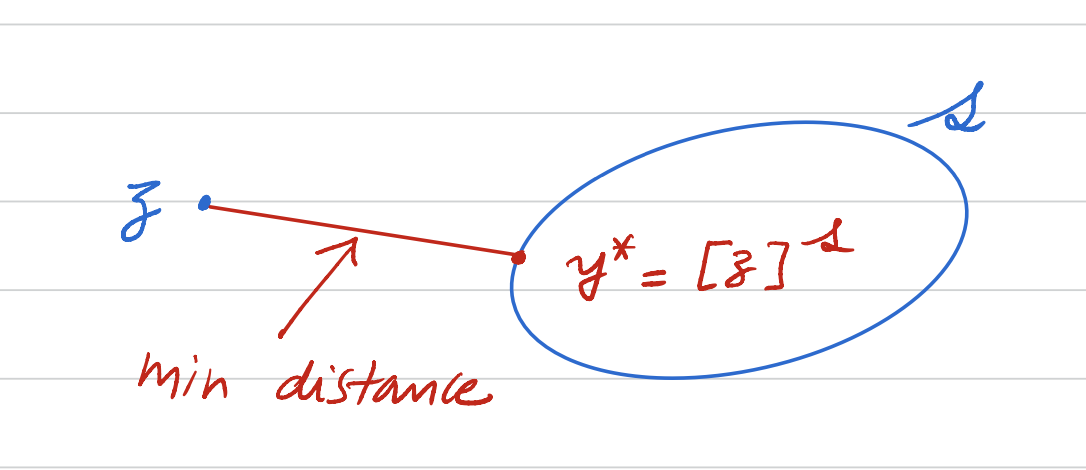
\includegraphics[scale=0.5]{projection1.png}
    \caption{Projection onto Closed Convex Set}
    \label{}
\end{figure}\end{center}
\textbf{Note:} $[z]^\&$ exists and is unique in convex $\&$, however, when $\&$ is not convex, $[z]^\&$ may not be unique.
\begin{center}\begin{figure}[htbp]
    \centering
    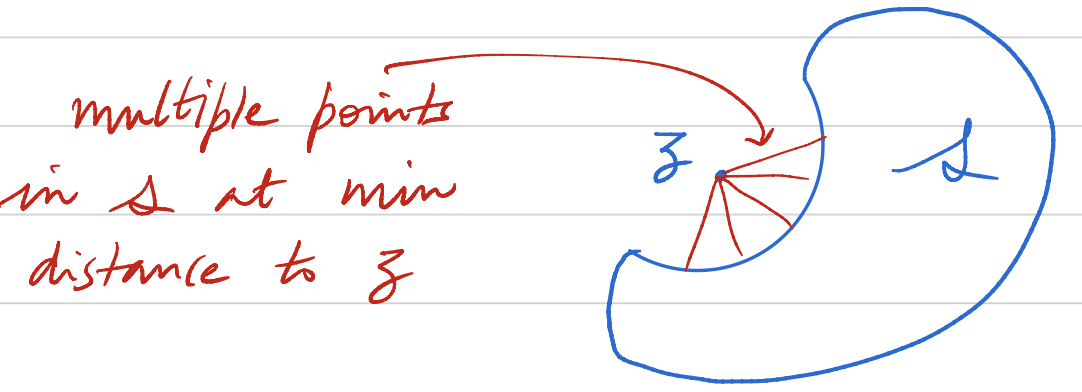
\includegraphics[scale=0.5]{projection2.png}
    \caption{Projection onto Closed non-Convex Set}
    \label{}
\end{figure}\end{center}

\subsection{Prop: \underline{unique} projection $[z]^\&$ on \underline{closed convex} subset of $\mathbb{R}^n$}
\begin{proposition}
    [Existence and Uniqueness of Projection]
    Let $\&$ be a \underline{closed convex} subset of $\mathbb{R}^n$. Then, for every $z\in \mathbb{R}^n$, there exists a unique $[z]^\&$.
\end{proposition}
\begin{proof}
Nee to show that $\min_{y\in \&}\|z-y\|^2$ exists and is unique.

Let $x$ be some element of $\&$. Then
\begin{equation}
    \begin{aligned}
        &\text{minimizing $\|z-y\|^2$ over all $y\in\&$}\\
        \equiv&\text{minimizing $\|z-y\|^2$ over the set $A=\{y\in\&:\|z-y\|^2\}$}
    \end{aligned}
    \nonumber
\end{equation}
$g(y)=\|z-y\|^2$ is strictly convex on set $\&$ $\Rightarrow$ $A$ is a convex set and $g$ is convex on $A$.

Also $g$ is continuous $\Rightarrow	A$ is closed.

Finally, $y\in A \Rightarrow \|y\|^2=\|y-z+z\|^2\leq \|y-z\|^2+\|z\|^2\leq \|z-x\|^2+\|z\|^2 \Rightarrow A$ is bounded.

Thus, $g(y)=\|z-y\|^2$ is strictly convex over set $A$, which is compact.

Therefore, $\min_{y\in\&}\|\&-y\|^2=\min_{y\in A}\|\&-y\|^2$ exists (Weierstrass’ Theorem) and is unique (strict convexity).
\end{proof}

\subsection{Obtuse Angle Criterion: $x=[z]^\&$ is projection on \underline{closed convex}subset of $\mathbb{R}^n$$\Leftrightarrow$ $(z-x)^T(y-x)\leq 0, \forall y\in\&$}

When solving the closest point problem for a vector space $S=\{\vec{y}:A \vec{y}=\vec{0}\}$ or affine subspace $S=\{\vec{y}:A \vec{y}=\vec{b}\}$, we use \textbf{perpendicularity condition} (orthogonality condition) -i.e., that $\vec{x}^*\cdot \vec{y}=0,\forall \vec{y}\in S$

A weaker form of that condition is the obtuse angle criterion, \textbf{which holds for any convex set}:
\begin{theorem}[Obtuse angle criterion]
    Let $C$ be a convex set and let $\vec{y}$ be a point outside $C$. $\vec{x}^*$ is the closest point in $C$ to $\vec{y}$ \underline{if and only if} $$(\vec{y}-\vec{x}^*)\cdot (\vec{x}-\vec{x}^*)\leq 0,\quad \forall \vec{x}\in C$$
\end{theorem}
\begin{center}\begin{figure}[htbp]
    \centering
    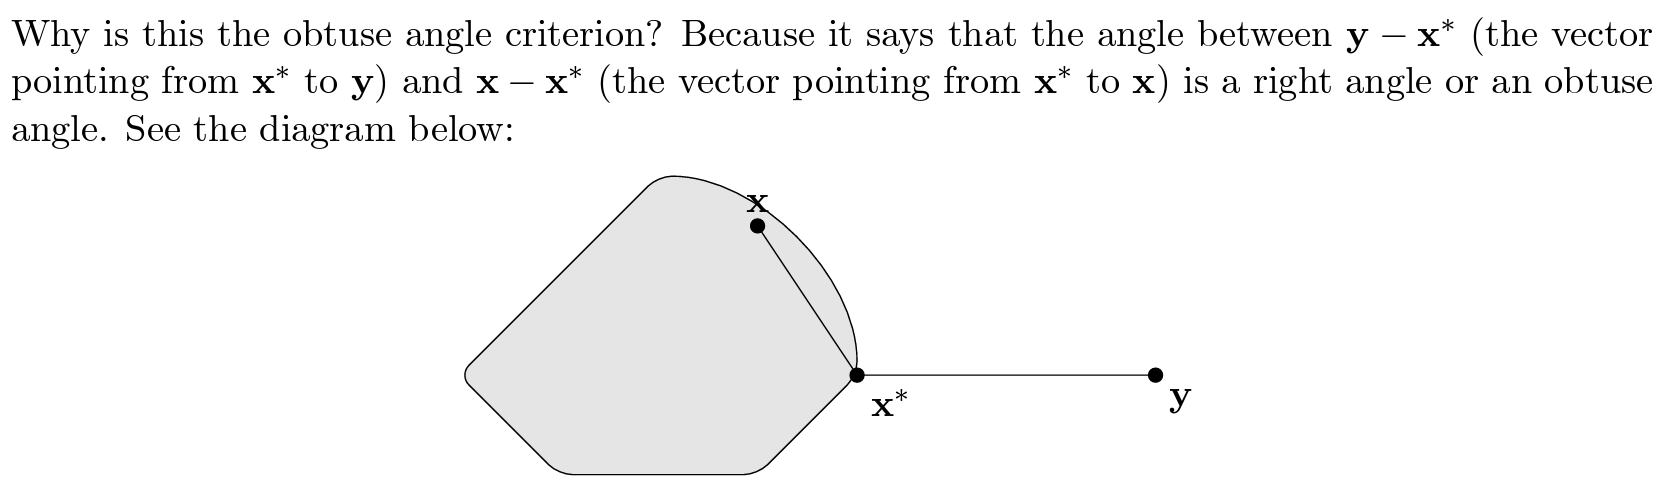
\includegraphics[scale=0.25]{obtuse.png}
    \caption{Obtuse angle criterion}
    \label{}
\end{figure}\end{center}
\textbf{In Projection Form}
\begin{proposition}
    [Necessary and Sufficient Condition for Projection]
    Let $\&$ be a \underline{closed conex} subset of $\mathbb{R}^n$. Then,
    \begin{equation}
        \begin{aligned}
            [z]^\&=y^*
            &\Leftrightarrow (y^*-z)^T(y-y^*)\geq 0,\quad \forall y\in\&.\\
            &\Leftrightarrow (z-y^*)^T(y-y^*)\leq 0,\quad \forall y\in\&.
        \end{aligned}
        \nonumber
    \end{equation}
\end{proposition}
\begin{proof}
    $[z]^\& = \argmin_{y\in\&}g(y)$, with $g(y)=\|z-y\|^2$ (which is strictly convex), $\nabla g(y)=2(y-z)$.

    By the optimality conditions,
    \begin{equation}
        \begin{aligned}
            &y^*\text{ is the unique minimizer of $g(y)$ over $\&$}\\
            \Leftrightarrow	& \nabla g(y^*)^T(y-y^*)\geq 0\quad \forall y\in\&\\
            \Leftrightarrow & (y^*-z)^T(y-y^*)\geq 0,\quad \forall y\in\&.\\
            \Leftrightarrow &(z-y^*)^T(y-y^*)\leq 0,\quad \forall y\in\&.
        \end{aligned}
        \nonumber
    \end{equation}
\end{proof}
\begin{center}\begin{figure}[htbp]
    \centering
    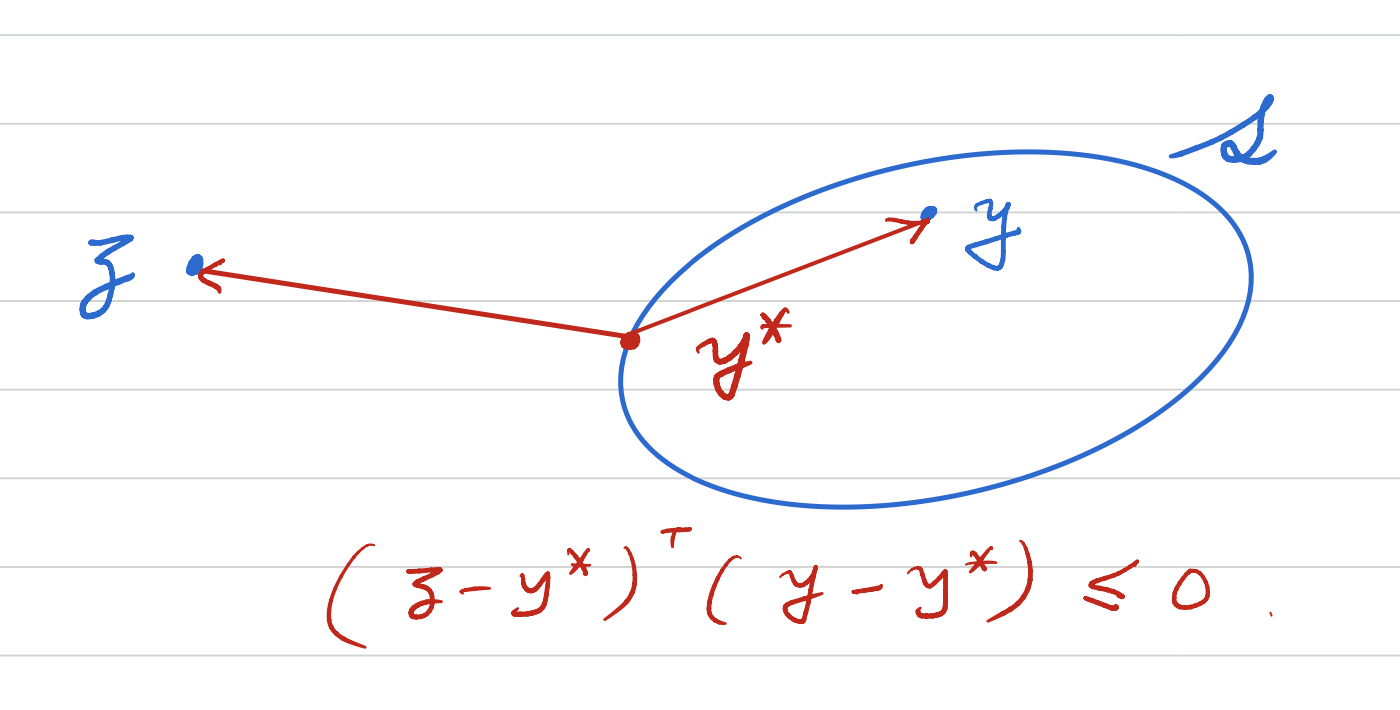
\includegraphics[scale=0.3]{projection3.png}
    \caption{Necessary and Sufficient Condition for Projection}
    \label{}
\end{figure}\end{center}

\subsection{Prop: Projection is non-expansive $\|[x]^\&-[z]^\&\|\leq \|x-z\|,\forall x,z\in \mathbb{R}^n$}
\begin{proposition}
    [Projection is non-expansive]
    Let $\&$ be a \underline{closed convex} subset of $\mathbb{R}^n$. Then for $x,z\in \mathbb{R}^n$
    $$\|[x]^\&-[z]^\&\|\leq \|x-z\|\quad \forall x,z\in \mathbb{R}^n$$
\end{proposition}
\begin{proof}
From previous theorem, we know
\begin{equation}
    \begin{aligned}
        (1).\quad ([x]^\&-x)^T(y-[x]^\&)\geq 0,\quad \forall y\in\&.\\
        (2).\quad ([z]^\&-z)^T(y-[z]^\&)\geq 0,\quad \forall y\in\&.\\
    \end{aligned}
    \nonumber
\end{equation}
set $y=[z]^\&$ in (1) and $y=[x]^\&$ in (2), and adding,
\begin{equation}
    \begin{aligned}
        &([z]^\&-[x]^\&)^T([x]^\&-x+z-[z]^\&)\geq 0\\
        \Rightarrow	& ([z]^\&-[x]^\&)^T(z-x)\geq \|[z]^\&-[x]^\&\|^2
    \end{aligned}
    \nonumber
\end{equation}
Applying Cauchy-schwary inequality,
\begin{equation}
    \begin{aligned}
        \|[z]^\&-[x]^\&\|^2&\leq \|[z]^\&-[x]^\&\|\|z-x\|\\
        \|[z]^\&-[x]^\&\|&\leq \|z-x\|
    \end{aligned}
    \nonumber
\end{equation}
\end{proof}

\section{Projection on (Linear) Subspaces of $\mathbb{R}^n$}
\subsection{Orthogonality Principle in subspaces of $\mathbb{R}^n$: $(z-y^*)^Tx= 0,\forall x\in\&$}
Suppose $\&$ is a linear subspace of $\mathbb{R}^n$, any linear combination of points in $\&$ is also in $\&$. Note that $\&$ is \underline{closed and convex}.

Then, for $z\in \mathbb{R}^n$, $[z]^\&=y^*$ satisfies:
\begin{equation}
    \begin{aligned}
        (z-y^*)^T(y-y^*)\leq 0,\quad \forall y\in\&.
    \end{aligned}
    \nonumber
\end{equation}
According to the property of subsapce, we can infer that
\begin{equation}
    \begin{aligned}
        (z-y^*)^Tx\leq 0,\quad \forall x\in\&.
    \end{aligned}
    \nonumber
\end{equation}
$-x$ also in $\&$, $-x\in\& \Rightarrow$
\begin{equation}
    \begin{aligned}
        (z-y^*)^Tx\geq 0,\quad \forall x\in\&.
    \end{aligned}
    \nonumber
\end{equation}
Then we can infer that
\begin{equation}
    \begin{aligned}
        (z-y^*)^Tx= 0,\quad \forall x\in\&.
    \end{aligned}
    \nonumber
\end{equation}
which is called \underline{orthogonality principle}.

\begin{center}\begin{figure}[htbp]
    \centering
    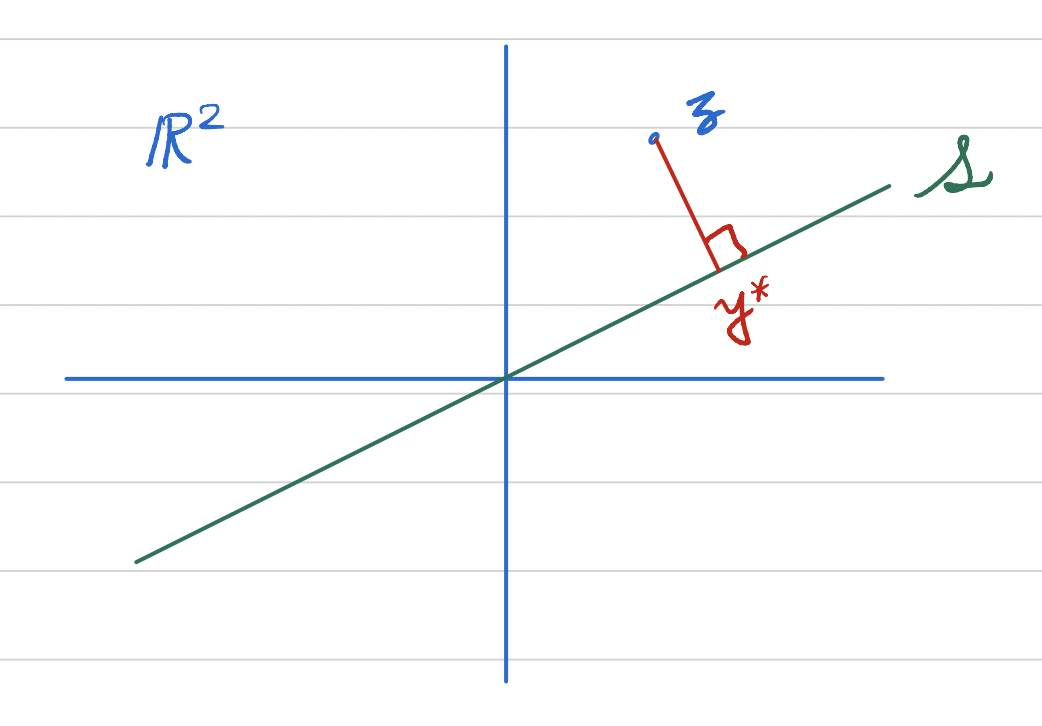
\includegraphics[scale=0.5]{proj1.png}
    \caption{Point from $\mathbb{R}^2$ to $\mathbb{R}$}
    \label{}
\end{figure}\end{center}











\section{Gradient Projection Method}
$\min_{x\in\&}f(x)$, $\&$ is convex and closed.
$$x_{k+1}=[x_k+\alpha_k d_k]^\&$$
\underline{Special Case}: Fixed step-size, steepest descent
\begin{equation}
    x_{k+1}=[x_k-\alpha \nabla f(x_k)]^\&
\end{equation}
\subsection{Def: \underline{fixed point} in fixed step-size steepest descent method, $\tilde{x}=[\tilde{x}-\alpha \nabla f(\tilde{x})]^\&$}
\begin{definition}
    $\tilde{x}$ is a \underline{fixed (stationary) point} of iteration in (1) if $$\tilde{x}=[\tilde{x}-\alpha \nabla f(\tilde{x})]^\&$$
\end{definition}

\subsection{Prop: $L-$smooth, $0<\alpha<\frac{2}{L}$ $\Rightarrow$ limit point is a fixed point (in fixed step-size steepest descent method)}
\begin{proposition}
    If $f$ has $L-$Lipschitz gradient and $0<\alpha<\frac{2}{L}$, every limit point of (1) is a fixed point of (1).
\end{proposition}
\begin{proof}
By the Descent Lemma,
\begin{equation}
    f(x_{k+1})\leq f(x_k)+\nabla f(x_k)^T(x_{k+1}-x_k)+\frac{L}{2}\|x_{k+1}-x_k\|^2
\end{equation}
By the necessary and sufficient condition for projection,
\begin{equation}
    (x_k-\alpha \nabla f(x_k)-x_{k+1})^T(x-x_{k+1})\leq 0,\quad \forall x\in\&
    \nonumber
\end{equation}
Set $x=x_k$ above
\begin{equation}
    \Rightarrow	\alpha \nabla f(x_k)^T(x_{k+1}-x_k)\leq -\|x_k-x_{k+1}\|^2
\end{equation}
According to (2) and (3), $$f(x_{k+1})-f(x_k)\leq (\frac{L}{2}-\frac{1}{\alpha})\|x_k-x_{k+1}\|^2$$ where $\frac{L}{2}-\frac{1}{\alpha}<0$

If $\{x_k\}$ has limit point $\bar{x}$, $LHS \stackrel{k \rightarrow \infty}{\longrightarrow}0$ $$\|x_{k+1}-x_{k}\|\stackrel{k \rightarrow \infty}{\longrightarrow}0 \Rightarrow [\bar{x}-\alpha \nabla f(\bar{x})]^\&=\bar{x}$$
\end{proof}

\subsection{Prop: $x$ is minimizer in convex func $\Leftrightarrow$ fixed point (in fixed step-size steepest descent method)}
\begin{proposition}
    If $f$ is convex, then $x^*$ is a minimizer of $f$ over $\&$ $\Leftrightarrow$ $x^*=[x^*-\alpha \nabla f(x^*)]^\&$ (i.e., $x^*$ is a fixed point of (1))
\end{proposition}
\begin{proof}
    \begin{equation}
        \begin{aligned}
            \text{$x^*$ is minimizer of convex $f$ over $\&$} &\Leftrightarrow \nabla f(x^*)^T(x-x^*)\geq 0,\forall x\in \&\\
            &\Leftrightarrow -\alpha\nabla f(x^*)^T(x-x^*)\leq 0,\forall x\in \&\\
            &\Leftrightarrow (x^*-\alpha\nabla f(x^*)-x^*)^T(x-x^*)\leq 0,\forall x\in \&\\
            \text{(By Projection Theorem)}&\Leftrightarrow [x^*-\alpha\nabla f(x^*)]^\&=x^*\\
        \end{aligned}
        \nonumber
    \end{equation}
\end{proof}

\subsection{Thm: Convergence of Gradient Projection: Convex, $L-$smooth, $0<\alpha<\frac{2}{L}$ $\Rightarrow$ $f(x_k)\rightarrow f(x^*)$ at rate $\frac{1}{k}$}
\begin{theorem}
    If $f$ is convex and $L-$Lipschitz gradient, it can be shown that for $0<\alpha<\frac{2}{L}$
    $$f(x_k)\rightarrow f(x^*)\text{ at rate }\frac{1}{k}\text{(same as unconstrainted)}$$
\end{theorem}

\subsection{Thm: Strongly convex, Lipschitz gradient $\Rightarrow$ $\{x_k\}$ converges to $x^*$ geometrically}
\begin{theorem}
    If $f$ has Lipschitz gradient with Lipschitz constant $M$ and strongly convex with parameter $m$, $\{x_k\}$ converges to $x^*$ \textbf{geometrically}.
\end{theorem}
\begin{proof}
$M-$smooth $\Rightarrow$ $$\|\nabla f(x)-\nabla f(y)\|\leq M\|x-y\|,\quad \forall x,y\in\&$$
$m-$strongly convex $\Rightarrow$
$$\nabla^2 f(x)\succeq mI,\quad \forall x\in\&$$
$$(x-y)^T(\nabla f(x)-\nabla f(y))\geq m\|x-y\|^2\quad \forall x,y\in\&$$
Let $x^*$ be the (unique) min of $f$ over $\&$
\begin{equation}
    \begin{aligned}
        \|x_{k+1}-x^*\|^2&=\|[x_k-\alpha \nabla f(x_k)]^\&-x^*\|^2\\
        (x^*\text{ is fixed point})\quad \quad &=\|[x_k-\alpha \nabla f(x_k)]^\&-[x^*-\alpha \nabla f(x^*)]^\&\|^2\\
        (\text{non-expansive})\quad \quad &\leq \|(x_k-\alpha \nabla f(x_k))-(x^*-\alpha \nabla f(x^*))\|^2\\
        &=\|(x_k-x^*)-\alpha( \nabla f(x_k)- \nabla f(x^*))\|^2\\
        &=\|x_k-x^*\|^2+\alpha^2\|\nabla f(x_k)-\nabla f(x^*)\|^2-2\alpha(x_k-x^*)^T(\nabla f(x_k)-\nabla f(x^*))\\
        (\nabla f\text{ is M-Lipschitz})\quad \quad &\leq \|x_k-x^*\|^2+\alpha^2M^2\|x_k-x^*\|^2-2\alpha(x_k-x^*)^T(\nabla f(x_k)-\nabla f(x^*))\\
        (m-\text{strong convexity})\quad &\leq \|x_k-x^*\|^2+\alpha^2M^2\|x_k-x^*\|^2-2\alpha m\|x_k-x^*\|^2\\
        &=(1+\alpha^2M^2-2\alpha m)\|x_k-x^*\|^2
    \end{aligned}
    \nonumber
\end{equation}
$$\|x_{k+1}-x^*\|^2\leq (1+\alpha^2M^2-2\alpha m)\|x_k-x^*\|^2$$
If $|1+\alpha^2M^2-2\alpha m|<1$. Then $x_N \rightarrow x^*$ \textbf{geometrically} as $N \rightarrow \infty$. (Same as unconstrained case)
\end{proof}










\chapter{(Unconstrained Optimization) Sub-gradient Methods}
Gradient descent methods require $\nabla f$ exists. What if $\nabla f$ doesn't exist at some point?

Recall that when $\nabla f$ exists

$f$ is convex on $\&$ $\Leftrightarrow f(y)\geq f(x)+\nabla f(x)^T(y-x),\forall x,y\in\&$ (the inequality is strict for strict convexity)
\section{Sub-gradient}
\begin{definition}
    For \underline{convex} $f$ on $\mathbb{R}^n$, $g$ is called a \textbf{sub-gradient} of $f$ at $x\in \mathbb{R}^n$ if $$f(y)\geq f(x)+g^T(y-x),\quad \forall y\in \mathbb{R}^n$$
\end{definition}
\subsection*{\underline{Properties of Sub-gradient}}
\begin{enumerate}[1)]
    \item Sub-gradient always exist at any point for convex functions.
    \item If $\nabla f$ exists at a point $x$ for convex $f$, sub-gradient is \underline{unique and $=\nabla f(x)$}
    \item Some definition for sub-gradient can be applied for non-convex $f$, but sub-gradient may not exist.
\end{enumerate}

\begin{example}
$f(x)=|x|,x\in \mathbb{R}$
\end{example}
For $x\neq 0$, $\nabla f$ exists and $=$ sub-gradient.\\
For $x=0$, any $g\in[-1,1]$ is a sub-gradient.
\begin{proof}\quad
\begin{enumerate}[(1)]
    \item For $y>0$, $f(y)=y\geq f(0)+gy=gy,\forall g\in[-1,1]$
    \item For $y<0$, $f(y)=-y\geq f(0)+gy=gy,\forall g\in[-1,1]$
\end{enumerate}
\end{proof}

\section{Sub-differential}
\begin{definition}
    Set of all sub-gradient at $x$ is called \textbf{sub-differential} at $x$, denoted $\partial f(x)$.
\end{definition}
\begin{example}
For $f(x)=|x|$,
\begin{equation}
    \begin{aligned}
        \partial f(x)=\left\{\begin{matrix}
            -1&\text{ if }x<0\\
            [-1,1]&\text{ if }x=0\\
            1&\text{ if }x>0\\
        \end{matrix}\right.
    \end{aligned}
    \nonumber
\end{equation}
\end{example}

\begin{example}
For $f(x)=\max\{1,|x|-1\}$. (Note: $f(x)$ is convex since $1,|x|-1$ are both convex.)
\begin{equation}
    \begin{aligned}
        \partial f(x)=\left\{\begin{matrix}
            -1&\text{ if }x<-2\\
            [-1,0]&\text{ if }x=-2\\
            0&\text{ if }-1<x<2\\
            [0,1]&\text{ if }x=2\\
            1&\text{ if }x>2\\
        \end{matrix}\right.
    \end{aligned}
    \nonumber
\end{equation}
\end{example}
When $x=2$,
\begin{equation}
    \begin{aligned}
        f(y)=\max\{1,|y|-1\}\geq f(2)+g(y-2)=1+g(y-2)
    \end{aligned}
    \nonumber
\end{equation}
\begin{enumerate}[(1)]
    \item \underline{$y\geq 0$}: $0\geq g(y-2)$ or $0\geq (g-1)(y-2)$. If $y>2$, $g\leq 1$; If $y=2$, $\forall g$; If $0\leq y< 2$, $g\geq 0$. $\Rightarrow g\in[0,1]$
    \item \underline{$y< 0$}: $0\geq g(y-2)$ or $-y-2\geq g(y-2)$, i.e. $g\geq 0$ or $g\leq \frac{2+y}{2-y}$ (satisifed by $g\in[0,1]$)
\end{enumerate}

\section{More examples}
\begin{example}
    $f(x)=\|x\|=\sqrt{x^Tx}$
\end{example}
\begin{enumerate}[$\bullet$]
    \item $f$ is convex (by Triangle Inequality: $\|x\|+\|y\|\geq \|x+y\|$)
    \item For $x\neq 0$, $\nabla f(x)$ exists and $$\partial f(x)= \nabla f(x) =\frac{1}{2\sqrt{x^Tx}}\cdot 2x=\frac{x}{\|x\|}$$
    \item If $x=0$, $\nabla f(x)$ doesn't exist.
\end{enumerate}

\begin{proposition}
    $\partial f(0)=\{g\in \mathbb{R}^n:\|g\|\leq 1\}$
\end{proposition}
\begin{proof}
    Need to show that for $\|g\|\leq 1$ and $\forall y\in \mathbb{R}^n$, $$f(y)=\|y\|\geq f(0)+g^T(y-0)=g^T y$$
    But by Cauchy-Schwarz inequality, for $\|g\|\leq 1$, $$g^Ty\leq \|g\|\|y\|\leq \|y\|,\forall y\in \mathbb{R}^n$$
    To estabilish the converse, suppose $\|g\|>1$.

    Then, setting $y=\frac{g}{\|g\|}$ $\Rightarrow$ $\|y\|=1$ but $g^Ty=\|g\|>1=\|y\|$
\end{proof}

\begin{example}
    $f(x)=|x_1-x_2|\leftarrow$ convex
\end{example}
If $x_1>x_2$, $|x_1-x_2|=x_1-x_2$, and $\nabla f$ exists and $(1,-1)$

If $x_1<x_2$, $|x_1-x_2|=x_2-x_1$, and $\nabla f$ exists and $(-1,1)$

\begin{proposition}
    If $x_1=x_2$, $\partial f(x)=\{(a,b):a=-b,|a|\leq 1\}$
\end{proposition}
\begin{proof}
    Suppose $x_1=x_2=c$. Then we need to show $\forall y\in \mathbb{R}^2$, $(a,b)$ s.t. $a=-b$, $|a|\leq 1$
    \begin{equation}
        \begin{aligned}
            |y_1-y_2|\geq f(c,c)+[a\ b]\begin{bmatrix}
                y_1-c\\
                y_2-c
            \end{bmatrix}=ay_1+by_2-c(a+b)=a(y_1-y_2)
        \end{aligned}
        \nonumber
    \end{equation}
    Since $|a|<1$, this inequality holds $\forall y\in \mathbb{R}^2$
    
    To show the converse,
    \begin{enumerate}
        \item Suppose $a\neq -b$.
        
        If $c(a+b)<0$, setting $y_1=y_2=0$. $\Rightarrow |y_1-y_2|=0$, and $ay_1+by_2-c(a+b)=-c(a+b)>0=|y_1-y_2|$, above inequality fails to hold.

        If $c(a+b)>0$, setting $y_1=y_2=2c$. $\Rightarrow |y_1-y_2|=0$, and $ay_1+by_2-c(a+b)=c(a+b)>0=|y_1-y_2|$, above inequality fails to hold.

        If $c=0$, setting $y_1=y_2=(a+b)$. $\Rightarrow |y_1-y_2|=0$, and $ay_1+by_2-c(a+b)=(a+b)^2>0=|y_1-y_2|$, above inequality fails to hold.
        \item Suppose $a=-b$ with $|a|>1$.
        
        If $a>1$, setting $y_1=y_2+1$; If $a<-1$, setting $y_1=y_2-1$.

    \end{enumerate}
\end{proof}

\section{First-order necessary conditions for optimality in terms of subgradient}
\begin{proposition}
    For convex $f$, $f(x^*)=\min_x f(x)\Leftrightarrow 0\in \partial f(x^*)$
\end{proposition}
\begin{proof}
    $x^*$ is a minimizer $\Leftrightarrow$ $f(x^*)\leq f(y),\forall y\in \mathbb{R}^n$ $\Leftrightarrow$ $f(x^*)+0^T(y-x^*)\leq f(y),\forall y\in \mathbb{R}^n$ $\Leftrightarrow$ $0\in \partial f(x^*)$
\end{proof}

\section{Properties of Subgradients}
Let $f,f_1,f_2$ be convex functions.
\begin{enumerate}[(a)]
    \item \textbf{Scaling:} For scalar $a > 0$, $\partial(af) = a\partial f$, i.e., $g$ is a subgradient of $f$ at $x$ if and only if $ag$ is a subgradient of af at $x$.
    \item \textbf{Addition:} If $g_1$ is a subgradient of $f_1$ at $x$, and $g_2$ is a subgradient of $f_2$ at $x$, then $g_1 + g_2$ is subgradient of $f_1 + f_2$ at $x$.
    \item \textbf{Affine Combination:} Let $h(x) = f(Ax+b)$, with $A$ being a square, invertible matrix. Then $\partial h(x) = A^T\partial f(Ax+b)$, i.e., $g$ is a subgradient of $f$ at $Ax + b$ if and only if $A^Tg$ is a subgradient of $h$ at $x$.
\end{enumerate}

\section{Sub-gradient Descent for Unconstrained Optimization}
\textbf{\underline{Assumptions:}}
\begin{enumerate}[(i)]
    \item $f$ is convex on $\mathbb{R}^n$.
    \item $f^*=\inf_{x\in \mathbb{R}^n}f(x)$ exists and there exists an $x^*$ s.t. $f(x^*)=f^*$.
    \item For all $x\in \mathbb{R}^n$ and for all $g\in \partial f(x)$, $\|g\|\leq a$.
\end{enumerate}
Subgradient Descent with constant step-size:
\begin{equation}
    \begin{aligned}
        x_{k+1}=x_k-\alpha g_k,\quad g_k\in \partial f(x_k)
    \end{aligned}
    \nonumber
\end{equation}
\textbf{\underline{Analysis:}}
\begin{equation}
    \begin{aligned}
        \|x_{k+1}-x^*\|^2&=\|x_k-\alpha g_k-x^*\|^2\\
        &=\|x_k-x^*\|^2+\alpha^2\|g_k\|^2-2\alpha g_k^T(x_k-x^*)\\
        &\leq \|x_k-x^*\|^2+\alpha^2a^2-2\alpha g_k^T(x_k-x^*)
    \end{aligned}
    \nonumber
\end{equation}
By the definition of $g_k$,
\begin{equation}
    \begin{aligned}
        &f(x_k)+g_k^T(x^*-x_k)\leq f(x^*)=f^*
    \end{aligned}
    \nonumber
\end{equation}
\begin{equation}
    \begin{aligned}
        \Rightarrow  \|x_{k+1}-x^*\|^2&\leq \|x_k-x^*\|^2+\alpha^2a^2+2\alpha (f^*-f(x_k))\\
        f(x_k)-f^*&\leq \frac{\|x_k-x^*\|^2-\|x_{k+1}-x^*\|^2+\alpha^2a^2}{2\alpha}
    \end{aligned}
    \nonumber
\end{equation}
Define $f_N^*=\min\{f(x_0),f(x_1),...,f(x_{N-1})\}$
\begin{equation}
    \begin{aligned}
        \sum_{k=0}^{N-1}(f(x_k)-f^*)\geq \sum_{k=0}^{N-1}(f_N^*-f^*)=N(f_N^*-f^*)
    \end{aligned}
    \nonumber
\end{equation}
Then,
\begin{equation}
    \begin{aligned}
        N(f_N^*-f^*)&\leq \sum_{k=0}^{N-1}\frac{\|x_k-x^*\|^2-\|x_{k+1}-x^*\|^2+\alpha^2a^2}{2\alpha}\\
        &=\frac{\|x_0-x^*\|^2-\|x_{N}-x^*\|^2+N\alpha^2a^2}{2\alpha}\\
        \Rightarrow\quad f_N^*&\leq f^*+\frac{1}{2\alpha N}\|x_0-x^*\|^2+\frac{\alpha a^2}{2}\\
        \lim_{N \rightarrow	\infty} f_N^*&\leq f^*+\frac{\alpha a^2}{2}
    \end{aligned}
    \nonumber
\end{equation}
For $\alpha$ samll enough and $N$ large enough $f^*_N$ can be made as close to $f^*$ as desired.

\subsection*{Note: $-$subgradient is not necessarily a descent direction}
i.e., if $g_k$ is a subgradient of $f$ at $x_k$. Then $$f(x_k-\alpha g_k)\text{ may be }\geq f(x_k),\quad \forall \alpha>0$$
for some $g_k$.

\begin{example}
    $f(x)=|x_1|+\frac{1}{2}x_2^2$
\end{example}
Suppose $x_k=(0,1)$, then it is easy to show: $\partial f(0,1)=([-1,1],1)$

Consider $g_k=(-1,1)\in\partial f(0,1)$
\begin{equation}
    \begin{aligned}
        f(x_k-\alpha g_k)=f(0+\alpha,1-\alpha)=\frac{1}{2}(1+\alpha^2)>\frac{1}{2}=f(x_k),\forall \alpha>0
    \end{aligned}
    \nonumber
\end{equation}
i.e., $-g_k$ is not a descent direction.

\begin{center}
    \fcolorbox{black}{gray!10}{\parbox{.9\linewidth}{If $f$ is convex, there is some $g_k\in\partial f(x_k)$ for which $-g_k$ is a descent direction (usually the one with \textbf{the smallest norm}), but finding such $g_k$ may be difficult in high-dimentional settings.\\ This means we cannot use back-tracking algorithms (Armijo's Rule) for adopting step-size.}}
\end{center}

\section{(Revised) Sub-gradient "descent" with diminishing stepsize}
\textbf{\underline{Assumptions:}}
\begin{enumerate}[(i)]
    \item $f$ is convex on $\mathbb{R}^n$.
    \item $f^*=\inf_{x\in \mathbb{R}^n}f(x)$ exists and there exists an $x^*$ s.t. $f(x^*)=f^*$.
    \item For all $x\in \mathbb{R}^n$ and for all $g\in \partial f(x)$, $\|g\|\leq a$.
\end{enumerate}
Subgradient Descent with constant step-size:
\begin{equation}
    \begin{aligned}
        x_{k+1}=x_k-\alpha_k g_k,\quad g_k\in \partial f(x_k)
    \end{aligned}
    \nonumber
\end{equation}
\textbf{\underline{Analysis:}}
\begin{equation}
    \begin{aligned}
        \|x_{k+1}-x^*\|^2&=\|x_k-\alpha_k g_k-x^*\|^2\\
        &=\|x_k-x^*\|^2+\alpha_k^2\|g_k\|^2-2\alpha_k g_k^T(x_k-x^*)\\
        &\leq \|x_k-x^*\|^2+\alpha_k^2a^2-2\alpha_k g_k^T(x_k-x^*)
    \end{aligned}
    \nonumber
\end{equation}
By the definition of $g_k$,
\begin{equation}
    \begin{aligned}
        &f(x_k)+g_k^T(x^*-x_k)\leq f(x^*)=f^*
    \end{aligned}
    \nonumber
\end{equation}
\begin{equation}
    \begin{aligned}
        \Rightarrow  \|x_{k+1}-x^*\|^2&\leq \|x_k-x^*\|^2+\alpha_k^2a^2+2\alpha_k (f^*-f(x_k))\\
        &\leq \left(\|x_{k-1}-x^*\|^2+\alpha_{k-1}^2a^2+2\alpha_{k-1}(f^*-f(x_{k-1}))\right)+\alpha_k^2a^2+2\alpha_k (f^*-f(x_k))\\
        &\dots\\
        \Rightarrow  \|x_{N}-x^*\|^2&\leq \|x_{0}-x^*\|^2+a^2\sum_{k=0}^{N-1}\alpha_{k}^2+2\sum_{k=0}^{N-1}\alpha_k(f^*-f(x_{k}))
    \end{aligned}
    \nonumber
\end{equation}
Define $f_N^*=\min\{f(x_0),f(x_1),...,f(x_{N-1})\}$
\begin{equation}
    \begin{aligned}
        \|x_{N}-x^*\|^2&\leq \|x_{0}-x^*\|^2+a^2\sum_{k=0}^{N-1}\alpha_{k}^2+2(f^*-f_N^*)\sum_{k=0}^{N-1}\alpha_k
    \end{aligned}
    \nonumber
\end{equation}
Then,
\begin{equation}
    \begin{aligned}
        f_N^*-f^*&\leq \frac{\|x_0-x^*\|^2-\|x_{N}-x^*\|^2+a^2\sum_{k=0}^{N-1}\alpha_k^2}{2\sum_{k=0}^{N-1}\alpha_k}\\
        &\leq \frac{\|x_0-x^*\|^2+a^2\sum_{k=0}^{N-1}\alpha_k^2}{2\sum_{k=0}^{N-1}\alpha_k}
    \end{aligned}
    \nonumber
\end{equation}
Suppse $\{\alpha_k\}$ is such that $\lim_{N \rightarrow	\infty}\frac{\sum_{k=0}^{N-1}\alpha_k^2}{\sum_{k=0}^{N-1}\alpha_k}=0$, then $\lim_{N \rightarrow \infty} f_N^*=f^*$

\subsection*{Example of $\{\alpha_k\}$ and convergence rate}
\begin{enumerate}[1)]
    \item $\alpha_k=\frac{1}{k+1},k=0,1,...$
    \begin{equation}
        \begin{aligned}
            &\sum_{k=0}^{N-1}\alpha_k^2=\sum_{k=1}^{N}\frac{1}{k^2}\rightarrow \frac{\pi^2}{6}\\
            &\sum_{k=0}^{N-1}\alpha_k=\sum_{k=1}^{N}\frac{1}{k}>\log N\\
            \Rightarrow&(f^*_N-f^*)\sim O(\frac{1}{\log N})
        \end{aligned}
        \nonumber
    \end{equation}
    \item $\alpha_k=\frac{1}{\sqrt{k+1}},k=0,1,...$
    \begin{equation}
        \begin{aligned}
            &\sum_{k=0}^{N-1}\alpha_k^2=\sum_{k=1}^{N}\frac{1}{k}<\log N+1\\
            &\sum_{k=0}^{N-1}\alpha_k=\sum_{k=1}^{N}\frac{1}{\sqrt{k}}>2\sqrt{N}-2\\
            \Rightarrow&(f^*_N-f^*)\sim O(\frac{\log N}{\sqrt{N}})
        \end{aligned}
        \nonumber
    \end{equation}
\end{enumerate}
Both worse than gradient descent (GD) $O(\frac{1}{N})$.

\chapter{(Unconstrained Optimization) Newton's Method}
\section{Classical Newton's Method}
\begin{definition}[Classical Newton's Method]
    One dimensional:

    Finding solution to non-linear equation:
    $$g(x^*)=0$$ with $g:\mathbb{R} \rightarrow \mathbb{R}$. Given $x_k$, find $x_{k+1}$ to solve $x^*$.
    \begin{equation}
        \begin{aligned}
            0=g(x_{k+1})\approx g(x_k)+g'(x_k)(x_{k+1}-x_k)
        \end{aligned}
        \nonumber
    \end{equation}
    Assuming $g'(x_k)\neq 0$, set
    \begin{equation}
        \begin{aligned}
            x_{k+1}=x_k-\frac{g(x_k)}{g'(x_k)}
        \end{aligned}
        \nonumber
    \end{equation}
\end{definition}
Similarly, when consider the minimizing problem of $f: \mathbb{R}^n \rightarrow \mathbb{R}$.
The Newton's method is $$\vec{x}_{k+1}=\vec{x}_k- \nabla g(\vec{x}_{k})^{-1}g(\vec{x}_k)$$



\section{Variants of Newton's Method}
\subsection{Generalization to Optimization}
In optimization, the goal is to get to $x$ s.t. $\nabla f(x)=0$.

Given $x_k$, we want to find $x_{k+1}$ s.t. $\nabla f(x_{k+1})=0$.

Taylor's Approx: \begin{equation}
    \begin{aligned}
        \nabla f(x_{k+1})\approx \nabla f(x_k)+\nabla^2 f(x_k)(x_{k+1}-x_k)
    \end{aligned}
    \nonumber
\end{equation}
Set $$x_{k+1}=x_k-(\nabla^2 f(x_k))^{-1}\nabla f(x_k)$$
which can be viewed as GD with $\alpha_k=1$ and $d_k=-(\nabla^2 f(x_k))^{-1}\nabla f(x_k)$

If $\nabla^2 f(x_k)\succeq 0$, then $\nabla f(x_k)^Td_k\geq 0$.

\subsection{The Secant Method}
The secant method is a replacement for ordinary Newton's method when we can't compute derivatives. In this case, we replace the derivative $f'(x_k)$ by the approximation $\frac{f(x_k)-f(x_{k-1})}{x_k-x_{k-1}}$ using the values of $f$ at the \textit{two} most recent points.

This gives us the iterative step
$$
x_{k+1}=x_k-\frac{f\left(x_k\right)}{\frac{f\left(x_k\right)-f\left(x_{k-1}\right)}{x_k-x_{k-1}}}=x_k-\frac{f\left(x_k\right)}{f\left(x_k\right)-f\left(x_{k-1}\right)}\left(x_k-x_{k-1}\right)
$$
which involves no derivatives. That's the secant method.

As we approach a solution $x^*, x_k$ and $x_{k-1}$ become very close to each other, and therefore $\frac{f\left(x_k\right)-f\left(x_{k-1}\right)}{x_k-x_{k-1}}$ is a very good approximation of $f^{\prime}\left(x_k\right)$ (or of $f^{\prime}\left(x_{k-1}\right)$ ). So we expect this method to perform almost as well as Newton's method (in cases where Newton's method does perform well).

We lose some efficiency, of course, because the approximation is not perfect. But the advantage is that we don't have to compute derivatives, so we can deal with a wider class of problems.



\section{A New Interpretation of Newton's Method}
Since $f(x)\approx f(x_k)+\nabla^T f(x_k)(x-x_k)+\frac{1}{2}(x-x_k)^T \nabla^2 f(x_k) (x-x_k)$, at each step $k$, we can solve a quadratic minimization problem,
\begin{equation}
    \begin{aligned}
        x_{k+1}=\argmin_{x\in \mathbb{R}^p}\{f(x_k)+\nabla^T f(x_k)(x-x_k)+\frac{1}{2}(x-x_k)^T \nabla^2 f(x_k) (x-x_k)\}
    \end{aligned}
    \nonumber
\end{equation}

\section{Convergence of Newton's Method}

\subsection{Guarantees of Convergence}
\begin{theorem}
    Suppose that we are using Newton's method to solve $g(\vec{x}) = \vec{0}$ for some $g : \mathbb{R}^n \rightarrow  \mathbb{R}^n$ (with continuous first partial derivatives). If the sequence of points $\vec{x}_1,\vec{x}_2,...$ that we get converges to some limit $\vec{x}^*$, then $g(\vec{x}^*) = \vec{0}$.

\end{theorem}
\subsection{Convergence Rate}
Let $x^*$ be s.t. $\nabla f(x^*)=0$, then
\begin{equation}
    \begin{aligned}
        \|x_{k+1}-x^*\|&=\|x_k-x^*-(\nabla^2 f(x_k))^{-1}\nabla f(x_k)\|\\
        &=\|x_k-x^*-(\nabla^2 f(x_k))^{-1}(\nabla f(x_k)-\nabla f(x^*))\|\\
    \end{aligned}
    \nonumber
\end{equation}
By Taylor's theorem,
\begin{equation}
    \begin{aligned}
        \nabla f(x_k)=\nabla f(x^*)+\nabla^2 f(x^*+\beta(x_k-x^*))(x_k-x^*)\text{ for some }\beta\in[0,1]
    \end{aligned}
    \nonumber
\end{equation}
Thus,
\begin{equation}
    \begin{aligned}
        \|x_{k+1}-x^*\|
        &=\|x_k-x^*-(\nabla^2 f(x_k))^{-1}\nabla^2 f(x^*+\beta(x_k-x^*))(x_k-x^*)\|\\
        &=\|(\nabla^2 f(x_k))^{-1}(\nabla^2 f(x^*+\beta(x_k-x^*))-\nabla^2 f(x_k))(x_k-x^*)\|\\
        &\leq \|(\nabla^2 f(x_k))^{-1}\|\|\nabla^2 f(x^*+\beta(x_k-x^*))-\nabla^2 f(x_k)\|\|x_k-x^*\|
    \end{aligned}
    \nonumber
\end{equation}
We use 1-norm $\|A\|=\max_{x\neq 0}\frac{\|Ax\|}{\|x\|}$ here, $\|A\|\geq \frac{\|Ax\|}{\|x\|} \Rightarrow	\|Ax\|\leq \|A\|\|x\|$.

Easy to prove, for symmetric $A\succeq 0$, $\|A\|=\lambda_{\max}(A)$, $\|A^{-1}\|=\lambda_{\max}(A^{-1})=\lambda^{-1}_{\min}(A)$

\begin{enumerate}[$\bullet$]
    \item Now suppose \textbf{\underline{$f$ is loacl $m$-strongly convex near $x^*$}}, then
    \begin{equation}
        \begin{aligned}
            \nabla^2 f(x^*)\succeq mI\text{ with }m>0\\
            \Rightarrow	\lambda_{\min}( \nabla^2 f(x^*))\geq m>0\\
            \Rightarrow	\lambda^{-1}_{\min}( \nabla^2 f(x^*))\leq \frac{1}{m}\\
        \end{aligned}
        \nonumber
    \end{equation}
    \item When $f$ is not local strongly convex near $x^*$. Assuming $\nabla^2 f(x)$ is continuous, if $\|x_k-x^*\|$ is small, then $\lambda_{\min}(\nabla^2 f(x_k))$ is close to $\lambda_{\min}(\nabla^2 f(x^*))$ i.e $\lambda_{\min}(\nabla^2 f(x^*))$ should be greater than a constant $\lambda_{\min}(\nabla^2 f(x^*))\geq \bar{\gamma}>0$. Then,
    \begin{equation}
        \begin{aligned}
            \|\nabla^2 f(x_k)^{-1}\|=\lambda^{-1}_{\min}(\nabla^2 f(x_k))\leq \frac{1}{\bar{\gamma}}=\gamma
        \end{aligned}
        \nonumber
    \end{equation}
\end{enumerate}

Furthurmore, \underline{assume that \textbf{$\nabla^2 f$ is L-Lipschitz in a neighborhood $\&$ of $x^*$}}, i.e.
\begin{equation}
    \begin{aligned}
        \|\nabla^2 f(x)-\nabla^2 f(y)\|\leq L\|x-y\|\quad \forall x,y\in \&
    \end{aligned}
    \nonumber
\end{equation}

Thus,
\begin{equation}
    \begin{aligned}
        \|x_{k+1}-x^*\|&\leq \|(\nabla^2 f(x_k))^{-1}\|\|\nabla^2 f(x^*+\beta(x_k-x^*))-\nabla^2 f(x_k)\|\|x_k-x^*\|\\
        &\leq \gamma L\|x^*+\beta(x_k-x^*)-x_k\|\|x_k-x^*\|\\
        &\leq \gamma L\|(\beta-1)(x_k-x^*)\|\|x_k-x^*\|\\
        \text{(Since $\beta\in [0,1]$)}\quad&\leq \gamma L\|x_k-x^*\|^2
    \end{aligned}
    \nonumber
\end{equation}
Hence,
\begin{equation}
    \begin{aligned}
        \|x_{k+1}-x^*\|\leq \gamma L\|x_k-x^*\|^2
    \end{aligned}
    \nonumber
\end{equation}
Now suppose \textbf{\underline{$x_0$ is close enough to $x^*$}} s.t.
\begin{equation}
    \begin{aligned}
        \gamma L\|x_0-x^*\|=\sigma<1
    \end{aligned}
    \nonumber
\end{equation}
Then,
\begin{equation}
    \begin{aligned}
        \|x_1-x^*\|&\leq \sigma\|x_0-x^*\|\\
        \|x_2-x^*\|&\leq \gamma L\|x_1-x^*\|^2\\
        &\leq \gamma L\sigma^2\|x_0-x^*\|^2=\sigma^3\|x_0-x^*\|\\
        \|x_3-x^*\|&\leq \gamma L\|x_2-x^*\|^2\\
        &\leq \gamma L\sigma^6\|x_0-x^*\|^2=\sigma^7\|x_0-x^*\|\\
        &\dots\\
        \|x_N-x^*\|&\leq \sigma^{2^N-1}\|x_0-x^*\|\\
    \end{aligned}
    \nonumber
\end{equation}
Assuming \textbf{\underline{$\nabla f$ is $M$-Lipschitz in neighborhood of $x^*$}},
\begin{equation}
    \begin{aligned}
        f(x_N)-f(x^*)&\leq \nabla f(x^*)(x_N-x^*)+\frac{M}{2}\|x_N-x^*\|^2\\
        &\leq \frac{M}{2}\sigma^{(2^{N+1}-2)}\|x_N-x^*\|^2\\
    \end{aligned}
    \nonumber
\end{equation}
Thus to make $f(x_N)-f(x^*)<\varepsilon$, need $N\sim O(log(log(\frac{1}{\varepsilon})))$

We call it \textbf{order-2 or super-linear convergence}.

\section{Note: Cons and Pros}
\begin{enumerate}[$\bullet$]
    \item Newton's Method is super-fast close to local min if function strongly convex around min.
    \item If the function is \underline{quadratic}, Newton's method converges in \underline{one step}.
    \begin{equation}
        \begin{aligned}
            f(x)=\frac{1}{2}x^TQx+bx+c,\quad Q\succ 0.\\
            \nabla f(x)=Qx+b,\nabla^2 f(x)=Q.\\
            \text{Global min $x^*$ satisfies } Qx^*+b=0 \Rightarrow	x^*=-Q^{-1}b
        \end{aligned}
        \nonumber
    \end{equation}
    Newton's method: for any $x_0\in \mathbb{R}^n$,
    \begin{equation}
        \begin{aligned}
            x_1&=x_0-(\nabla^2 f(x_0))^{-1}\nabla f(x_0)\\
            &=x_0-Q^{-1}(Qx_0+b)=-Q^{-1}b=x^*
        \end{aligned}
        \nonumber
    \end{equation}
    \textbf{Intuition:} when $f$ is a quadratic function, $\nabla^3 f(x)=0, \forall x$. Hence, $f(x)= f(x_k)+\nabla^T f(x_k)(x-x_k)+\frac{1}{2}(x-x_k)^T \nabla^2 f(x_k) (x-x_k)$, the minimization problem will get the min in one step.
    \item But Newton's method has several \textbf{drawbacks}:
    \begin{enumerate}[(1)]
        \item Newton’s method requires the matrix inversion step, and this is quite expensive. So the \underline{per step cost for Newton’s method is higher}.
        \item Newton’s method has faster local convergence but \underline{may diverge} if initialized from some place far from the optimal point.
        \item $\nabla^2 f(x)^{-1}$ may fail to exist, i.e. $\nabla^2 f(x)$ is singular, e.g. linear $f$.
        \item It is not necessarily a general GD method since $\nabla^2 f(x_k)$ may not be $\succ 0$.
        \item It is not a descent method, $f(x_{k+1})$ may be $> f(x_k)$.
        \item It may stop at local max or saddle points.
    \end{enumerate}
\end{enumerate}

\section{Modifications to ensure global convergence}
\begin{enumerate}[(a)]
    \item Try Newton's method. If either $\nabla^2 f(x_k)$ is singular or $f(x_{k+1})>f(x_{k})$ then use (b).
    \item Find $\delta_k$ s.t. $$(\delta_k I+\nabla^2 f(x_k))\succ 0$$ and $$\lambda_{\min}(\delta_k I+\nabla^2 f(x_k))\succeq \Delta >0$$ so that $\delta_k I+\nabla^2 f(x_k)$ is easily invertible.
    
    Then set $d_k=-(\delta_k I+\nabla^2 f(x_k))^{-1}\nabla f(x_k)$. This ensures that $\nabla^T f(x_k)d_k<0$.

    Then we use $x_{k+1}=x_k+\alpha_k d_k$ with $\alpha_k$ chosen using Armijo's Rule.

    If at any point $\nabla^2 f(x_k)\succ 0$, go back to Newton's method and check if $f(x_{k+1})<f(x_k)$. Continue Newton's method as long as $\nabla^2 f(x_k)\succ 0$ and $f(x_{k+1})<f(x_{k})$.
\end{enumerate}

\section{Quasi-Newton Methods}
Estimating Hessian $\nabla^2 f(x_k)$ is expensive, so we use some simplier matrix $H_k$ instead.

Quasi-Newton method have the iteration form:
\begin{equation}
    \begin{aligned}
        x_{k+1}=x_k-\alpha_kH_k^{-1}\nabla f(x_k)
    \end{aligned}
    \nonumber
\end{equation}
where $H_k$ is some estimated version of $\nabla^2 f(x_k)$, and the stepsize $\alpha_k$ is typically determined by Armijo rule.

Previously, we approximate $f(x)$ by
$$f(x)\approx f(x_k)+\nabla^T f(x_k)(x-x_k)+\frac{1}{2}(x-x_k)^T \nabla^2 f(x_k) (x-x_k)$$
Now, we define the form by $H_k$
$$g(x)=f(x_k)+\nabla^T f(x_k)(x-x_k)+\frac{1}{2}(x-x_k)^T H_k (x-x_k)$$
We hope $g(x)\approx f(x)$ and optimize $g$ for this step. We enforce
\begin{enumerate}[(1)]
    \item $\nabla f(x_k)=\nabla g(x_k)$\quad  (Automatically satisfied)
    \item $\nabla f(x_{k-1})=\nabla g(x_{k-1})$\quad $\Leftrightarrow$\quad $$H_k(x_k-x_{k-1})=\nabla f(x_k)-\nabla f(x_{k-1})$$
\end{enumerate}
The condition $(2)$ is called the \underline{secant equation}.

There are infinitely many $H_k$ satisfying this condition. Various choices of $H_k$ lead to different Quasi-Newton methods. We discuss the BFGS method.

\subsection{BFGS Method}
We need $H_k$ to be constructed in a way that it can be efficiently computed.

We want $H_k$ to have two properties:
\begin{enumerate}[$(1)$]
    \item $H_k$ can be computed by some iterative formula $$H_k=H_{k-1}+M_{k-1}$$
    \item $H_k$ is positive definite (at least guarantee that the BFGS method is a descent method, i.e. $f(x_{k+1})\leq f(x_k)$).
\end{enumerate}
We can choose $H_0>0$ and then guarantee $M_k\geq 0$.

\textbf{Rank-2 BFGS Method}:
\begin{equation}
    \begin{aligned}
        H_{k+1}=H_k+a_kv_kv_k^T+b_ku_ku_k^T
    \end{aligned}
    \nonumber
\end{equation}
where $v_k\in \mathbb{R}^p$ and $u_k\in \mathbb{R}^p$ are some vectors. If $H_0>0$, the above iterative formula can guarantee $H_k$ to be positive definite.

How can we choose $v_k$ and $u_k$ to guarantee the secant equation $H_{k+1}(x_{k+1}-x_{k})=\nabla f(x_{k+1})-\nabla f(x_{k})$?

Let's denote $s_k=x_{k+1}-x_k$ and $y_k=\nabla f(x_{k+1})-\nabla f(x_k)$. The secant equation: $H_{k+1}s_k=y_k$, then substitute it into the above formula,
\begin{equation}
    \begin{aligned}
        y_{k}=H_{k+1}s_k&=H_ks_k+a_k v_k v_k^T s_k+b_ku_ku_k^Ts_k\\
        \Leftrightarrow y_{k}-H_ks_k&=a_k (v_k^T s_k)v_k+b_k(u_k^Ts_k)u_k\\
    \end{aligned}
    \nonumber
\end{equation}
To let the above equation be satisfied. We let $v_k=y_k$, $u_k=H_k s_k$, $a_k=\frac{1}{y_k^T s_k}$, and $b_k=-\frac{1}{s_k^TH_ks_k}$. Then, the iteration formula becomes
\begin{center}
    \fcolorbox{black}{gray!10}{\parbox{.9\linewidth}{\begin{equation}
        \begin{aligned}
            H_{k+1}=H_k+\frac{y_ky_k^T}{y_k^T s_k}-\frac{H_k s_ks_k^TH_k}{s_k^TH_ks_k}
        \end{aligned}
        \nonumber
    \end{equation}
    where $s_k=x_{k+1}-x_k$ and $y_k=\nabla f(x_{k+1})-\nabla f(x_k)$.}}
\end{center}

This is exactly the BFGS method.

Since we implement the BFGS method as
\begin{equation}
    \begin{aligned}
        x_{k+1}=x_k-\alpha_k H_k^{-1}\nabla f(x_k)
    \end{aligned}
    \nonumber
\end{equation}
It will be better to compute $H_{k}^{-1}$ directly instead of $H_k$.
\begin{equation}
    \begin{aligned}
        H_{k+1}^{-1}&=\left(H_k+\frac{y_ky_k^T}{y_k^T s_k}-\frac{H_k s_ks_k^TH_k}{s_k^TH_ks_k}\right)^{-1}\\
        &=\left(H_k+[H_ks_k\ y_k]
        \begin{bmatrix}
            -\frac{1}{s_k^TH_ks_k}&0\\
            0&\frac{1}{y_k^Ts_k}
        \end{bmatrix}
        \begin{bmatrix}
            s_k^TH_k\\
            y_k^T
        \end{bmatrix}\right)^{-1}\\
        &\text{(by woodbury formula)}\\
        &=H_k^{-1}-H_k^{-1}[H_ks_k\ y_k]\left(\begin{bmatrix}
            -\frac{1}{s_k^TH_ks_k}&0\\
            0&\frac{1}{y_k^Ts_k}
        \end{bmatrix}^{-1}+
        \begin{bmatrix}
            s_k^TH_k\\
            y_k^T
        \end{bmatrix}H_k^{-1}[H_ks_k\ y_k]\right)^{-1}\begin{bmatrix}
            s_k^TH_k\\
            y_k^T
        \end{bmatrix}H_k^{-1}\\
        &=H_k^{-1}-[s_k\ H_k^{-1}y_k]\begin{bmatrix}
            0&s_k^Ty_k\\
            y_k^Ts_k&y_k^T(s_k+H_k^{-1}y_k)
        \end{bmatrix}^{-1}\begin{bmatrix}
            s_k^T\\
            y_k^TH_k^{-1}
        \end{bmatrix}\\
        &=H_k^{-1}-[s_k\ H_k^{-1}y_k]\begin{bmatrix}
            -\frac{y_k^Ts_k+y^T_kH_k^{-1}y_k}{y_k^Ts_ks_k^Ty_k}&\frac{1}{y_k^Ts_k}\\
            \frac{1}{y_k^Ts_k}&0
        \end{bmatrix}\begin{bmatrix}
            s_k^T\\
            y_k^TH_k^{-1}
        \end{bmatrix}\\
        &=H_k^{-1}-\frac{H_k^{-1}y_ks^T_k}{y_k^Ts_K}-\frac{s_ky^T_kH_k^{-1}}{y_k^Ts_K}+\frac{s_ks_k^T}{y_k^Ts_K}+\frac{s_ky_k^TH_k^{-1}y_ks_k^T}{(y_k^Ts_k)^2}\\
        &=\left(I-\frac{s_ky_k^T}{y^T_ks_k}\right)H_k^{-1}\left(I-\frac{y_ks_k^T}{y^T_ks_k}\right)+\frac{s_ks_k^T}{y^T_ks_k}
    \end{aligned}
    \nonumber
\end{equation}
\begin{center}
     \fcolorbox{black}{gray!10}{\parbox{.9\linewidth}{$$H_{k+1}^{-1}=\left(I-\frac{s_ky_k^T}{y^T_ks_k}\right)H_k^{-1}\left(I-\frac{y_ks_k^T}{y^T_ks_k}\right)+\frac{s_ks_k^T}{y^T_ks_k}$$  is the iteration computation $H_k^{-1}$ of BFGS method. where $s_k=x_{k+1}-x_k$ and $y_k=\nabla f(x_{k+1})-\nabla f(x_k)$.}}
\end{center}

\section{Trust-Region Method}
\begin{equation}
    \begin{aligned}
        x_{k+1}=\argmin_{\|x-x_k\|\leq\Delta_k}\{f(x_k)+\nabla^T f(x_k)(x-x_k)+\frac{1}{2}(x-x_k)^T \nabla^2 f(x_k) (x-x_k)\}
    \end{aligned}
    \nonumber
\end{equation}
This method can escape addle points under some assumptions.

\section{Cubic Regularization}
Contain higher order term $\|x-x_k\|^3$ to the quadratic estimation.


\chapter{(Constrained Optimization) Barrier Method}
\section{Barrier Method}
Computationed method to solve inequality constrained problems.
\begin{align*}
    &\min\quad f(x)\\
    &\begin{array}{r@{\quad}r@{}l@{\quad}l}
    s.t.
    &x\in\&&\\
    &g(x)\leq 0&\\
\end{array}
\end{align*}
where $\&$ is closed set.
\subsection*{Barrier Function}
$B(x)$ is a function that is continuous and $\rightarrow \infty$ as any $g_j(x) \rightarrow	0$
\begin{example}

    \begin{equation}
        \begin{aligned}
            B(x)&=-\sum_{j=1}^r\ln(-g_j(x))\\
            B(x)&=-\sum_{j=1}^r\frac{1}{g_j(x)}
        \end{aligned}
        \nonumber
    \end{equation}

\end{example}
\textbf{Note:} that if $g_j(x)$ is \underline{convex} for all $j$, then both of these barrier functions are \underline{convex}.

In Barrier Method, choose sequence $\{\varepsilon_k\}$ s.t.
\begin{equation}
    \begin{aligned}
        0<\varepsilon_{k+1}<\varepsilon_k,\quad k=0,1,...
    \end{aligned}
    \nonumber
\end{equation}
and $\varepsilon_k \rightarrow 0$ as $k \rightarrow	\infty$.

Define feasible set $F=\&\cap\{g_j(x)\leq 0,\forall j\}$. Note $F$ is a closed set since $\&$ and $\{g_j(x)\leq 0,\forall j\}$ are closed.

Let $x^{(k)}$ be a solution to
\begin{equation}
    \begin{aligned}
        \min_{x\in F\cap \text{dom}(B)}f(x)+\varepsilon_k B(x)
    \end{aligned}
    \nonumber
\end{equation}
Since $B(x) \rightarrow	\infty$ as one $g_j(x) \rightarrow	0$ which is on the boundary of $F$.

$x^{(k)}$ must be an interior point of $F$
$$\Rightarrow \nabla f(x^{(k)})+\varepsilon_k \nabla B(x^{(k)})=0$$
Therefore, if we have a initial point in the interior of $F$, we can choose step size of any unconstrained GD method to stay in interior of $F$ for all iterations and solve the ICP. (Because barrier function $B(x)$ will prevent us from reaching boundary)

As $k \rightarrow \infty$, $\varepsilon_k \rightarrow 0$, and barrier $\varepsilon_k B(x)$ becomes inconsequential, and we expect $x^{(k)}$ to approcah minimum of original problem.

\begin{proposition}
    Every limit point $\bar{x}$ of $\{x^{(k)}\}$ is a global min of the ICP.
\end{proposition}
\begin{proof}
Let $\bar{x}=\lim_{k \rightarrow \infty, k\in \mathcal{K}}x^{(k)}$, since $x^{(k)}\in F$ forall $k$, and $F$ is closed, $\bar{x}\in F$.

Suppose $x^*$ is a global min of ICP and $x^*$ is in interior of $F$, and $f(x^*)<f(\bar{x})$, i.e., $\bar{x}$ is not global min for ICP.

Then, by definition of $x^{(k)}$, $f(x^{(k)})+\varepsilon_k B(x^{(k)})\leq f(x^*)+\varepsilon_k B(x^*)$

Taking limit as $k \rightarrow \infty$, $k\in \mathcal{K}$,
\begin{equation}
    \begin{aligned}
        f(\bar{x})+\lim_{k \rightarrow \infty, k\in \mathcal{K}}\varepsilon_k B(\bar{x})\leq f(x^*)+\lim_{k \rightarrow \infty, k\in \mathcal{K}}\varepsilon_k B(x^*)=f(x^*)\\
        (\text{Since }|B(x^*)|<\infty,\varepsilon_k \rightarrow	0\text{ as }k \rightarrow \infty)
    \end{aligned}
    \nonumber
\end{equation}
If $\bar{x}$ is in interior of $F$, then $|B(\bar{x})|<\infty$ $\Rightarrow \lim_{k \rightarrow \infty, k\in \mathcal{K}}\varepsilon_k B(x^{(k)})=0$

If $\bar{x}$ is on boundary of $F$, then $|B(\bar{x})| \rightarrow \infty$ $\Rightarrow \lim_{k \rightarrow \infty, k\in \mathcal{K}}\varepsilon_k B(x^{(k)})\geq 0$

Therefore, $f(\bar{x})<f(x^*)$ is contradiced.

If $x^*$ is not in interior of $F$, we can assume that $\exists$ an interior point $\bar{x}$ which can be made arbitrarily close to $x^*$.
\end{proof}


\section{An Exmaple Using KKT or Barrier}
\begin{example}
\begin{equation}
    \begin{aligned}
        \min\quad&f(x)=\frac{1}{2}(x_1^2+x_2^2)\\
        s.t.\ & x_1\geq 2
    \end{aligned}
    \nonumber
\end{equation}
\end{example}
\subsection{Solution using KKT conditions}
\begin{equation}
    \begin{aligned}
        g(x)&=-x_1+2\\
        \nabla g(x)&=(-1,0)\quad \text{All feasible $x$ are regular}\\
        \nabla f(x)&=(x_1,x_2)\\
        L(x,\mu)&=f(x)+\mu g(x)\\
        \nabla L(x,\mu)&=\nabla f(x)+\mu \nabla g(x)=(x_1-\mu,x_2)\\
    \end{aligned}
    \nonumber
\end{equation}
\begin{enumerate}[\underline{Case} $1$:]
    \item constraint inactive, i.e., $\mu=0$
    $$\nabla L(x,\mu)=0 \Rightarrow	x=(0,0)$$
    Doesn't satisfy $x_1\geq 2$. This case is infeasible.
    \item constraint active,
    \begin{equation}
        \begin{aligned}
            \nabla L(x,\mu)=0 \Rightarrow x_1-\mu=0,x_2=0\\
            g(x)=0 \Rightarrow x_1=2\\
            \Rightarrow	x^*=(2,0), \mu=2
        \end{aligned}
        \nonumber
    \end{equation}
    It satisfies the first-order KKT condition.
\end{enumerate}
Since $L(x,\mu)$ is strictly convex on $\mathbb{R}^2$, $x^*=(2,0)$ is the global-min.

\subsection{Solution using logarithmic barrier}
$B(x)=-\ln(-g(x))=-\ln(x_1-2)$
\begin{equation}
    \begin{aligned}
        \text{Set }G^{(k)}(x)&=f(x)+\varepsilon_kB(x)\\
        &=\frac{1}{2}(x_1^2+x_2^2)-\varepsilon_k\ln(x_1-2)\\
        (G^{(k)}(x)&\text{ is convex in $x$ over }\{x:x>2\})\\
        \nabla G^{(k)}(x)=0 &\Rightarrow\ x_1-\frac{\varepsilon_k}{x_1-2}=0,\ x_2=0\\
        &\Rightarrow\ x^{(k)}=(1+\sqrt{1+\varepsilon_k},0)\\
        \text{as }k \rightarrow	\infty,\varepsilon_k \rightarrow 0&\text{ and }x^{(k)} \rightarrow (2,0)=x^*
    \end{aligned}
    \nonumber
\end{equation}

\section{Penalty Method (For ECP)}
Computational method for \underline{equality constraints}.
\begin{equation}
    \begin{aligned}
        \min\quad &f(x)\\
        s.t.\ &x\in \&\\
        &h_i(x)=0,\quad i=1,...,m
    \end{aligned}
    \nonumber
\end{equation}
\subsection*{\underline{Algorithm}}
\begin{enumerate}[(1)]
    \item Choose an increasing positive sequence $\{c_k\}$ s.t. $c_k \rightarrow \infty$ as $k \rightarrow \infty$.
    \item Solve for $x^{(k)}$ to:
    \begin{equation}
        \begin{aligned}
            \min_{x\in \&}\quad &f(x)+c_k\|h(x)\|^2\\
            \text{Note: } &\|h(x)\|^2=\sum_{i=1}^m(h_i(x))^2
        \end{aligned}
        \nonumber
    \end{equation}
\end{enumerate}
\begin{proposition}
    Every limit point $\bar{x}$ of $\{x^{(k)}\}$ is a global min of the ECP if $\&$ is closed.
\end{proposition}
\begin{proof}
    Let $\bar{x}=\lim_{k \rightarrow \infty, k\in \mathcal{K}}x^{(k)}$
    \begin{equation}
        \begin{aligned}
            f^*&=\min_{x\in\&,h(x)=0}f(x)=\min_{x\in\&,h(x)=0}f(x)+c_k\|h(x)\|^2\\
            &\geq \min_{x\in\&}f(x)+c_k\|h(x)\|^2\\
            &=f(x^{(k)})+c_k\|h(x^{(k)})\|^2\\
            \Rightarrow	c_k\|h(x^{(k)})\|^2&\leq f^*-f(x^{(k)})
        \end{aligned}
        \nonumber
    \end{equation}
    By continunity of $f$, $\lim_{k \rightarrow \infty, k\in \mathcal{K}}f(x^{(k)})=f(\bar{x})$.

    Thus, as $k \rightarrow	\infty$, $k \rightarrow	\mathcal{K}$, $f^*-f(x^{(k)})=f^*-f(\bar{x})$ which is \underline{finite}.

    Since $c_k \rightarrow \infty$ as $k \rightarrow	\infty$, $k \rightarrow	\mathcal{K}$, $$\lim_{k \rightarrow \infty, k\in \mathcal{K}}\|h(x^{(k)})\|^2=0$$

    By continunity of $h$,
    $$\lim_{k \rightarrow \infty, k\in \mathcal{K}}\|h(x^{(k)})\|^2=\|h(\bar{x})\|^2=0 \Rightarrow	h(\bar{x})=0$$

    Now, since $\&$ is closed, and $x^{(k)}\in \&$ for all $k$, $\bar{x}\in\&$ as well.

    \begin{equation}
        \begin{aligned}
            &f^*-f(x^{(k)})\geq c_k\|h(x^{(k)})\|^2\geq 0\\
            \Rightarrow	& f(\bar{x})=\lim_{k \rightarrow \infty, k\in \mathcal{K}}f(x^{(k)})\leq f^*
        \end{aligned}
        \nonumber
    \end{equation}
    Since $\bar{x}$ is feasible ($\bar{x}\in\&$ and $h(\bar{x})=0$) and $f(\bar{x})\leq f^*$, $\Rightarrow$ $\bar{x}$ is a global min of the ECP.
\end{proof}


\chapter{General Descent Method}
To minimize $f$, we want:
\begin{enumerate}
    \item Pick a direction to go in where f is decreasing.
    \item Go in that direction far enough to notice, but not too far.
\end{enumerate}

\section{Criteria for a descent method}
Our general iteration step from a point $x^{(k)}$ is to go to a point
$$x^{(k+1)}=x^{(k)}+t_k \vec{p}^{(k)}$$


\textbf{Criteria 1:} $f(x^{(k+1)})<f(x^{(k)})$

\textbf{Criteria 2:} $\vec{p}^{(k)}\cdot \nabla f(x^{(k)})<0$ (equivalent to $\phi'_k(0)<0$)

Let $\phi_k(t)=f(x^{(k)}+t \vec{p}^{(k)})$, $\phi'_k(t)=\vec{p}^{(k)}\cdot \nabla f(x^{(k)}+t \vec{p}^{(k)})$ the Criteria 2 asks $\phi'_k(0)<0$

\textbf{Criteria 3:} For some parameter $\beta\in (0,1)$, we have $\phi'_k(t_k)\geq \beta\phi'_k(0)$. ("don't take steps that are too small".)

If $t_k$ is close to $0$, $\phi'_k(t_k)$ will be close $\beta\phi'_k(0)$ with large negative. We don't want to waste a step at a $t_k$ close to $0$.

The value of $\beta$ is a parameter that measures how much we care about this criterion.

If we set $\beta=0$, the method goes back to the method of the steepest descent. This
criterion would tell us to keep going until we reach (or go past) a critical point of $\phi_k$.

If we set $\beta=1$, the criterion doesn't exist.

\textbf{Criteria 4:} For some parameter $\alpha\in (0,\beta)$, we have $\phi_k(t_k)\leq \phi_k(0)+\alpha t_k\phi'_k(0)$. ("only keep going for as long as you're getting at least a fraction of the promised
payoff".)

With Criteria 2 and 4, we can forget about Criteria 1 (which is a consequence of Criteria 2 and 4).

\section{Wolfe's theorem}
\begin{theorem}[Wolfe's theorem]
    Let $\alpha,\beta$ be real numbers satisfying $0 <\alpha < \beta < 1$. Assume $f : \mathbb{R}^n \rightarrow \mathbb{R}$ has continuous $\nabla f$ and is \underline{bounded below}. Starting from a point $x^{(k)}$, whenever $p^{(k)}$ \underline{satisfies Criterion 2} (it is a descent direction), then there is a range $[a_k, b_k]$ (with $0 < a_k < b_k$) such that for any $t_k \in [a_k, b_k]$, all four criteria are satisfied.
\end{theorem}




















\end{document}